\documentclass[9pt]{article}
% *** GRAPHICS RELATED PACKAGES ***
%
% \ifCLASSINFOpdf
%   % \usepackage[pdftex]{graphicx}
%   % declare the path(s) where your graphic files are
%   % \graphicspath{{../pdf/}{../jpeg/}}
%   % and their extensions so you won't have to specify these with
%   % every instance of \includegraphics
%   % \DeclareGraphicsExtensions{.pdf,.jpeg,.png}
% \else
%   % or other class option (dvipsone, dvipdf, if not using dvips). graphicx
%   % will default to the driver specified in the system graphics.cfg if no
%   % driver is specified.
%   % \usepackage[dvips]{graphicx}
%   % declare the path(s) where your graphic files are
%   % \graphicspath{{../eps/}}
%   % and their extensions so you won't have to specify these with
%   % every instance of \includegraphics
%   % \DeclareGraphicsExtensions{.eps}
% \fi

\usepackage{hyperref}
\usepackage{stfloats}



%% The amssymb package provides various useful mathematical symbols
\usepackage{amssymb}
\usepackage{framed,multirow}
\usepackage{url,microtype}
\usepackage{mathrsfs,bm} % Notacion de transformadas
\usepackage{amsmath}
\usepackage{amsfonts,eucal}
\usepackage[normalem]{ulem}

\usepackage{epsfig}
\usepackage{epstopdf}
\usepackage{booktabs}
\usepackage{adjustbox}
\usepackage[]{subfigure}
\usepackage{lineno}

\usepackage{tikz}
\usepackage{pgfplots}
%\usetikzlibrary{shadings}
\pgfplotsset{compat=1.16}
%\usetikzlibrary{arrows,shapes,shadows,calc,decorations.pathreplacing,positioning}
%\usetikzlibrary{spy}
\usepgfplotslibrary{fillbetween}

\usepackage{times}
%\usepackage[titletoc,toc,title]{appendix}
\usepackage{natbib}
\usepackage{float}
\usepackage[ruled,linesnumbered]{algorithm2e}
\usepackage{array}
\usepackage{color}
\usepackage[capitalize]{cleveref}
\usepackage{enumerate,multirow}
% \usepackage{lineno}


%%Defining some useful variables 
\providecommand{\promedd}[2]{\mathbb{E}_{#1}\!$\left\{#2\right\}$}% operador de promedio
\providecommand{\ve}[1]{{\bm{#1}}}%
\providecommand{\tr}[1]{{\operatorname{tr}$\left({#1}\right)$}}
\providecommand{\mat}[1]{{\bm{#1}}} %
\providecommand{\var}[1]{${\operatorname{var}}\left\{#1\right\}$}
\newcommand{\Real}{\mathbb{R}}
\newcommand{\N}{\mathbb{N}}
\newcommand{\Z}{\mathbb{Z}}

\DeclareMathOperator{\subconj}{\negthinspace\subset\negthinspace }
\DeclareMathOperator{\en}{\!\,\in\!\,}
\DeclareMathOperator{\igual}{\!\,=\!\,}
\DeclareMathOperator{\dist}{\operatorname{d}}
\DeclareMathOperator{\xx}{\negthickspace\times\negthickspace}
\providecommand{\s}[1]{\negthinspace#1\negthinspace}%

\renewcommand{\refname}{\normalsize References}
\newcommand{\dif}[1]{\mathrm{d}#1}
\newcommand{\Erf}[1]{\mathrm{erf}\left(#1\right)}
\newcommand{\Cov}[1]{\mathrm{cov}\left(#1\right)}
\newcommand{\sign}[1]{\mathrm{sign}(#1)}
\newcommand{\phivec}{\boldsymbol{\phi}}
\newcommand{\muvec}{\boldsymbol{\mu}}
\newcommand{\wfunc}[1]{\textnormal{w}(#1)}
\newcommand{\ex}[1]{\mathbb{E}[#1]}
\providecommand{\ve}[1]{{\mathbf{#1}}}

\DeclareMathOperator{\vecO}{vec} % vec operator
\providecommand{\mat}[1]{{\mathbf{#1}}}
\DeclareMathOperator{\cov}{cov} % Operator for the covariance
\DeclareMathOperator{\KL}{KL} % Operator for the KL divergence
\newcommand{\boldk}{\mathbf{k}} % kernel or covariance
\newcommand{\boldt}{\mathbf{t}} % kernel or covariance
\newcommand{\boldK}{\mathbf{K}} % kernel or covariance
\newcommand{\boldB}{\mathbf{B}} % coregionalization matrix
\newcommand{\boldA}{\mathbf{A}} % matrix of coeffcients a_{qi}^r
\newcommand{\boldc}{\mathbf{c}} % matrix of coeffcients a_{qi}^r
\newcommand{\boldu}{\mathbf{u}} % vector for latent function
\newcommand{\bolda}{\mathbf{a}}
\newcommand{\boldm}{\mathbf{m}}
\newcommand{\boldv}{\mathbf{v}}
\newcommand{\boldV}{\mathbf{V}}
\newcommand{\boldW}{\mathbf{W}}
\newcommand{\boldZ}{\mathbf{Z}}
\newcommand{\boldz}{\mathbf{z}}
\newcommand{\boldAtilde}{\mathbf{\widetilde{A}}}
\newcommand{\eye}{\mathbf{I}}   % identity matrix
\newcommand{\boldI}{\mathbf{I}} % identity matrix
\newcommand{\boldUpsi}{\bm{\Upsilon}}
\newcommand{\boldH}{\mathbf{H}} % The whole set of lag vectors
\newcommand{\inputSpace}{\mathcal{X}} % The input space
\newcommand{\params}{\bm{\theta}} % Parameters of LMC model
\newcommand{\veC}{\textbf{\hspace{-0.001in}:}} % Simplified version of the vec operator (vec = :)
\newcommand{\preci}{\mathbf{P}}% Precision for the Gaussians
\newcommand{\dataset}{{\cal D}} % dataset
\newcommand{\fracpartial}[2]{\frac{\partial #1}{\partial  #2}} % Fraction for partial derivatives
\newcommand{\gauss}{\mathcal{N}} % Gaussian density
\newcommand{\bolds}{\mathbf{s}}


\newcommand\redsout{\bgroup\markoverwith{\textcolor{red}{\rule[0.5ex]{2pt}{0.4pt}}}\ULon}
\providecommand{\roj}[1]{\textcolor{red}{\uwave{#1}}}
\providecommand{\ver}[1]{\textcolor{green}{\uwave{#1}}}
\providecommand{\gc}[1]{\textcolor{darkgray}{\uwave{#1}}}
\providecommand{\am}[1]{\textcolor[rgb]{0.1,0.5,0.0}{\upshape{#1}}}
% Leave a blank line between paragraphs instead of using \\

%Comments
\providecommand{\am}[1]{\textcolor[rgb]{0.1,0.5,0.0}{\upshape{#1}}}

\newcolumntype{C}[1]{>{\centering\let\newline\\\arraybackslash\hspace{0pt}}m{#1}}

\usepackage{pifont}% http://ctan.org/pkg/pifont
\newcommand{\cmark}{\ding{51}}%
\newcommand{\xmark}{\ding{55}}%
\usetikzlibrary{bayesnet}

% correct bad hyphenation here
\hyphenation{op-tical net-works semi-conduc-tor}

\newcommand{\comment}[2]{{\color{blue}#1} {\color{red}#2}}
% \AtBeginEnvironment{appendices}{\crefalias{section}{appendix}}
\textwidth 6.8 in
\oddsidemargin -0.2 in
\topmargin -0.5 in
\textheight 9 in
\footskip 0.35 in
\setlength{\parindent}{0in}

\begin{document}
\title{Correlated Chained Gaussian Processes with Multiple Annotators\\
Supplementary Material}
%
%
% author names and IEEE memberships
% note positions of commas and nonbreaking spaces ( ~ ) LaTeX will not break
% a structure at a ~ so this keeps an author's name from being broken across
% two lines.
% use \thanks{} to gain access to the first footnote area
% a separate \thanks must be used for each paragraph as LaTeX2e's \thanks
% was not built to handle multiple paragraphs
%

\author{J. Gil-Gonz\'alez,
        J. Giraldo,
        A. \'Alvarez-Meza, A. Orozco-Guti\'errez,  and~M.~A.~\'Alvarez% <-this % stops a space
}
\date{}


\maketitle

\section{Derivation of CCGPMA lower bounds}
\begin{align}
\notag\log p(\mat{Y}) &\igual\log \int p(\mat{Y}|\hat{\ve{f}})p(\hat{\ve{f}}|\ve{u})p(\ve{u})d\hat{\ve{f}} d\ve{u},\\
&\igual\log \int \prod_{j=1}^{J}p(\ve{f}_j|\ve{u})q(\ve{u}) \displaystyle\frac{p(\mat{Y}|\hat{\ve{f}})\displaystyle\prod_{j=1}^{J}p(\ve{f}_j|\ve{u})p(\ve{u})}{\displaystyle\prod_{j=1}^{J}p(\ve{f}_j|\ve{u})q(\ve{u})}d\hat{\ve{f}} d\ve{u}.
\end{align}
Using Jensen's inequality, we obtain
\begin{align}
 \log p(\mat{Y}) \ge &   \int \left(\prod_{j=1}^{J}p(\ve{f}_j|\ve{u})q(\ve{u})\right)\log\left(\frac{p(\mat{Y}|\hat{\ve{f}})\displaystyle\prod_{j=1}^{J}p(\ve{f}_j|\ve{u})p(\ve{u})}{\displaystyle\prod_{j=1}^{J}p(\ve{f}_j|\ve{u})q(\ve{u})}\right)d\hat{\ve{f}} d\ve{u},\\ 
\mathcal{L} \igual &  \prod_{j=1}^{J}\int q(\ve{f}_j)\log p(\mat{Y}|\hat{\ve{f}})d\hat{\ve{f}} -  \sum_{q=1}^{Q}\mathbb{D}_{KL}(q(\ve{u}_q)||p(\ve{u}_q)),
\label{eq:LowBound}
\end{align}
where $\mathbb{D}_{KL}(\cdot||\cdot)$ is the Kullback-Leibler--(KL) divergence and $q(\ve{f}_j)$ is defined as follows:
\begin{align}
 q(\ve{f}_j) &\igual \int p(\ve{f}_j|\ve{u})q(\ve{u})d\ve{u} \igual \gauss(\ve{f}_j|\bm{\mu}_j,\mat{S}_j),
\end{align}
where
\begin{align}
     \bm{\mu}_j &\igual \mat{K}_{\ve{f}_j\ve{u}}\mat{K}_{\ve{u}\ve{u}}^{-1}\ve{m},\\
     \mat{S}_j &\igual \mat{K}_{\ve{f}_j\ve{f}_j}+\mat{K}_{\ve{f}_j\ve{u}}\mat{K}_{\ve{u}\ve{u}}^{-1}(\mat{V}-\mat{K}_{\ve{u}\ve{u}})\mat{K}_{\ve{u}\ve{u}}^{-1}\mat{K}_{\ve{u}\ve{f}_j}.
\end{align}
Moreover, note that the solution of variational expectation (analytical or numerical)
\begin{align}
    \mathbb{E}_{\prod\limits^J_{j=1}q(f_j(\ve{x}_n))}\left[\log p(\mat{Y}|\hat{\ve{f}})\right]\igual \prod_{j=1}^{J}\int q(\ve{f}_j)\log p(\mat{Y}|\hat{\ve{f}})d\hat{\ve{f}}
\end{align}
will depend on the form of the likelihood $p(\mat{Y}|\hat{\ve{f}})$. For numerical solution, we will use Gaussian-Hermite quadratures. Thus, considering for simplicity an univariate case, the expectations can be approximated as
\begin{align}
\mathbb{E}_{q({f}_j)}\left[\log p(\mat{Y}|{f}_j)\right] \approx \frac{1}{\sqrt{\pi}}\sum_{s=1}^{S}w_s\log p(\mat{Y}|\sqrt{2{s}_j}{g}_s + {\mu}_j),
\end{align}
where ${\mu}_j$ and ${s}_j$ are respectively the mean and the variance of the distribution $q({f}_j)$. Besides, the pair of values $w_s$ and ${g}_s$ are obtained form the Hermite polynomial $H_n(x) = (-1)^ne^{x^2}\frac{d}{dx^n}e^{-x^2}$.

\subsection{Gradients w.r.t. the variational parameters} 
the idea is to maximize the lower bound in \cref{eq:LowBound} with respect to the variational parameters $\ve{m}_q$ and $\mat{V}_q$ of each distribution $q(\ve{u}_q)$. 

\textbf{Useful Equalities}: These equalities \cite{hensman2015scalable} are useful to compute the gradients 
\begin{align}
\fracpartial{}{\mu}\mathbb{E}_{\gauss(x|\mu,\sigma^2)}\left[h(x)\right] = \mathbb{E}_{\gauss(x|\mu,\sigma^2)}\left[\fracpartial{}{x}h(x)\right].\\
\fracpartial{}{\sigma^2}\mathbb{E}_{\gauss(x|\mu,\sigma^2)}\left[h(x)\right] = \frac{1}{2}\mathbb{E}_{\gauss(x|\mu,\sigma^2)}\left[\fracpartial{^2}{x^2}h(x)\right].
\end{align}
First, the bound derivatives w.r.t $\ve{m}_q$.
\begin{align}
\fracpartial{\mathcal{L}}{\ve{m}_q} &\igual \underbrace{\fracpartial{}{\ve{m}_q}\mathbb{E}_{q(\hat{\ve{f}})}\left[\log p(\mat{Y}|\hat{\ve{f}})\right]}_{\mbox{Variational Expectation--(VE) part}} - \fracpartial{}{\ve{m}_q}\underbrace{\sum_{q=1}^{Q}\mathbb{D}_{KL}(q(\ve{u}_q)||p(\ve{u}_q))}_{\mbox{KL part}},
\end{align}
where the KL part w.r.t. $\ve{m}_q$ yields
\begin{align}
\fracpartial{}{\ve{m}_q}{\mathbb{D}_{KL}(q(\ve{u}_q)||p(\ve{u}_q))} = \mat{K}_{\ve{u}_q\ve{u}_q}^{-1}\ve{m}_q.
\end{align}
Now, the VE part w.r.t. $\ve{m}_q$ is given as 
\begin{align}
\notag\fracpartial{}{\ve{m}_q}\mathbb{E}_{q(\hat{\ve{f}})}\left[\log p(\mat{Y}|\hat{\ve{f}})\right] &= \fracpartial{}{\ve{m}_q}\mathbb{E}_{q(\hat{\ve{f}})}\left[\log p(\mat{Y}|\hat{\ve{f}})\right],\\
\notag&\quad\; \mbox{Chain Rule:}\; \bm{\mu}_j=h(\ve{m}_q),\\
&= \underbrace{\mathbb{E}_{q(\hat{\ve{f}})}\left[\fracpartial{}{\hat{\ve{f}}}\log p(\mat{Y}|\hat{\ve{f}})\right]}_{\mbox{See Likelihoods}} \fracpartial{\bm{\mu}_j}{\ve{m}_q}.
\end{align}
Then, the bound derivatives w.r.t $\mat{V}_q$
\begin{align}
\fracpartial{\mathcal{L}}{\mat{V}_q} &\igual \underbrace{\fracpartial{}{\mat{V}_q}\mathbb{E}_{q(\hat{\ve{f}})}\left[\log p(\mat{Y}|\hat{\ve{f}})\right]}_{\mbox{VE part}} - \fracpartial{}{\mat{V}_q}\underbrace{\sum_{q=1}^{Q}\mathbb{D}_{KL}(q(\ve{u}_q)||p(\ve{u}_q))}_{\mbox{KL part}},
\end{align}
where the KL part w.r.t. $\mat{V}_q$ yields
\begin{align*}
\fracpartial{}{\mat{V}_q}{\mathbb{D}_{KL}(q(\ve{u}_q)||p(\ve{u}_q))} = \frac{1}{2}\left(\mat{K}_{\ve{u}_q\ve{u}_q}^{-1} - \mat{V}_q^{-1} \right).
\end{align*}
Now, the VE part w.r.t. $\mat{V}_q$ is given as 
\begin{align}
\notag\fracpartial{}{\mat{V}_q}\mathbb{E}_{q(\hat{\ve{f}})}\left[\log p(\mat{Y}|\hat{\ve{f}})\right] &= \fracpartial{}{\mat{V}_q}\mathbb{E}_{q(\hat{\ve{f}})}\left[\log p(\mat{Y}|\hat{\ve{f}})\right],\\
\notag &\quad\;\mbox{Chain Rule:}\;\ve{s}_j=h(\mat{V}_q),\\
&= \frac{1}{2}\underbrace{\mathbb{E}_{q(\hat{\ve{f}})}\left[\fracpartial{^2}{\hat{\ve{f}}^2}\log p(\mat{Y}|\hat{\ve{f}})\right]}_{\mbox{See Likelihoods}} \fracpartial{\ve{s}_j}{\mat{V}_q},
\end{align}
where $\ve{s}_j\en \Real^{N}$ is a vector containing the diagonal elements of matrix $\mat{S}_j$. On the other hand, the gradients w.r.t. the hyper-parameters are similar to the ones in \cite{moreno2018heterogeneous}. 
\section{Likelihood functions}\label{sec:LikeliFunc}
The models exposed previously accept a wide variety of likelihood functions $p(\mat{Y}|\hat{\ve{f}})$ \citep{saul2016chained}. To incorporate any new likelihood, we need to compute the following expressions:
\begin{enumerate}
	\item The likelihood $ p(\mat{Y}|\hat{\ve{f}})$.
	\item The Log-likelihood $\log p(\mat{Y}|\hat{\ve{f}})$.
	\item The variational expectation $\mathbb{E}_{q(\hat{\ve{f}})}\left[\log p(\mat{Y}|\hat{\ve{f}})\right]$.
	\item The first order derivatives $\fracpartial{}{\hat{\ve{f}}}\left[\log p(\mat{Y}|\hat{\ve{f}})\right]$.
	\item The variational expectation of first order derivatives $\mathbb{E}_{q(\hat{\ve{f}})}\left[\fracpartial{}{\hat{\ve{f}}}\left[\log p(\mat{Y}|\hat{\ve{f}})\right]\right]$.
	\item The second order derivatives $\fracpartial{^2}{\hat{\ve{f}}^2}\left[\log p(\mat{Y}|\hat{\ve{f}})\right]$.
	\item The variational expectation of second order derivatives $\mathbb{E}_{q(\hat{\ve{f}})}\left[\fracpartial{^2}{\hat{\ve{f}}^2}\left[\log p(\mat{Y}|\hat{\ve{f}})\right]\right]$.
	\item The predictive mean and variance.
\end{enumerate}

\subsection{Gaussian distribution for regression with multiple annotators}
For real-valued outputs, e.g., $\mathcal{Y} \s{\subset}\Real$, we follow the multi-annotator model used in \cite{raykar2010learning,groot2011learning,xiao2013learning,rodrigues2017learning}, where each output $y_n^r$ is considered to be a corrupted version of the hidden ground truth $y_n$.
\begin{enumerate}
	\item $ p(\mat{Y}|\hat{\ve{f}})$
	\begin{align}
	p(\mat{Y}|\hat{\ve{f}}) = \prod_{n=1}^{N}\prod_{r\in R_n}\gauss(y_n^r|y_n,v_n^r), 
	\end{align}
	where, $y_n = f_1(\ve{x}_n)$, and $v_n^r = \exp(f_{l_r}(\ve{x}_n))$, with $r\in \left\{1, \dots R\right\}$, and $l_r = r+1 \in \left\{2, \dots J\right\}$; hence, the number of required LFs are $J=R+1$.
	\item $\log p(\mat{Y}|\hat{\ve{f}})$
	\begin{align}
	\notag \log p(\mat{Y}|\hat{\ve{f}}) & = \log \prod_{n=1}^{N}\prod_{r\in R_n}\gauss(y_n^r|y_n,v_n^r), \\
	&= -\frac{1}{2}\sum_{n=1}^{N}\sum_{r\in R_n} \left\{\log(2\pi) + \log(v_n^r) + \frac{(y_n^r - y_n)^2}{v_n^r}  \right\},
	\end{align}
	where $\log v_n^r = \log (\exp(f_{l_r,n})) = f_{l_r,n}$
	\item $\mathbb{E}_{q(\hat{\ve{f}})}\left[\log p(\mat{Y}|\hat{\ve{f}})\right]$
	\begin{align}
	\notag \mathbb{E}_{q(\hat{\ve{f}})}\left[\log p(\mat{Y}|\hat{\ve{f}})\right] &=\int \prod_{j=1}^{J}q(\hat{\ve{f}}_j)\log p(\mat{Y}|\hat{\ve{f}})d\hat{\ve{f}}, \\
	&=\sum_{n=1}^{N}\sum_{r\in R_n}\mathbb{E}_{q(f_{1,n})q(f_{l_r,n})}\left[\log \gauss(y_n^r|y_n,v_n^r)\right].
	\end{align}
	Since $q(f_{1,n})$ and $q(f_{l_r,1})$ obey Gaussian distributions, the above integrals can be solved analytically as in \cite{lazaro2011variational}. Thus, we have
	{
		\begin{align}
		\notag\int q(f_{1,n})q(f_{l_r,n})&\log \gauss(y_n^r|y_n,v_n^r)df_{1,n} df_{l_r,n}\\ 
		&= \log \gauss\left(y_n^r|\mu_{1,n}, \exp\left({\mu_{l_r,n}-\frac{s_{l_r,n}}{2}}\right)\right) - \frac{s_{l_r,n}}{4} - \frac{s_{1,n}\exp\left(-\mu_{l_r,n} + \frac{s_{l_r,n}}{2} \right)}{2}.
		\end{align}}
	Thus, 
	\begin{align}
	\mathbb{E}_{q(\hat{\ve{f}})}\left[\log p(\mat{Y}|\hat{\ve{f}})\right] = \sum_{n=1}^{N}\sum_{r\in R_n}\log \gauss\left(y_n^r|\mu_{1,n}, \exp\left({\mu_{l_r,n}-\frac{s_{l_r,n}}{2}}\right)\right) - \frac{s_{l_r,n}}{4} - \frac{s_{1,n}\exp\left(-\mu_{l_r,n} + \frac{s_{l_r,n}}{2} \right)}{2},
	\end{align}
	where $f_{1,n}$ is the $n$-th position of vector $\ve{f}_1$, $f_{l_r,n}$ is the $n$-th position of vector $\ve{f}_{l_r}$, $\mu_{1,n}$ is the $n$-th position of vector $\muvec_1$, $\mu_{l_r,n}$ is the $n$-th position of vector $\muvec_{l_r}$, $s_{1,n}$ is the $n$-th position of vector $\ve{s}_{1}$, and $s_{l_r,n}$ is the $n$-th position of vector $\ve{s}_{l_r}$.
	\item $\fracpartial{}{\hat{\ve{f}}}\left[\log p(\mat{Y}|\hat{\ve{f}})\right]$
	\begin{align}
	\fracpartial{}{\hat{\ve{f}}}\left[\log p(\mat{Y}|\hat{\ve{f}})\right] = \fracpartial{}{\hat{\ve{f}}}\left[-\frac{1}{2}\sum_{n=1}^{N}\sum_{r\in R_n} \left\{\log(2\pi) + f_{l_r,n} + \frac{(y_n^r - f_{1,n})^2}{\exp(f_{l_r,n})}  \right\}\right].
	\end{align}
	\begin{description}
		\item[Case 1]
		\begin{align}
		\fracpartial{}{f_{1,n}}\left[-\frac{1}{2}\sum_{n=1}^{N}\sum_{r\in R_n} \left\{\frac{(y_n^r - f_{1,n})^2}{\exp(f_{l_r,n})}  \right\}\right] = \sum_{r\in R_n}\frac{(y_n^r - f_{1,n})}{\exp(f_{l_r,n})}.
		\end{align}
		\item[Case 2]
		\begin{align}
		\fracpartial{}{f_{l_r,n}}\left[-\frac{1}{2}\sum_{n=1}^{N}\sum_{r\in R_n} \left\{ + f_{l_r,n} + \frac{(y_n^r - f_{1,n})^2}{\exp(f_{l_r,n})}  \right\}\right] = \begin{cases}
		-\frac{1}{2} + \frac{(y_n^r - f_{1,n})^2}{2\exp(f_{l_r,n})}, & \mbox{if $r\in R_n$}\\
		0, & \mbox{Otherwise}
		\end{cases}.
		\end{align}
	\end{description}
	\item $\mathbb{E}_{q(\hat{\ve{f}})}\left[\fracpartial{}{\hat{\ve{f}}}\left[\log p(\mat{Y}|\hat{\ve{f}})\right]\right]$


	\begin{description}
		\item[Case 1] 
		\begin{align}
		\notag \mathbb{E}_{q(\hat{\ve{f}})}\left[\fracpartial{}{f_{1,n}}\left[\log p(\mat{Y}|\hat{\ve{f}})\right]\right] &= \sum_{r\in R_n}\mathbb{E}_{q(f_{1,n})q(f_{l_r,n})}\left[\frac{(y_n^r - f_{1,n})}{\exp(f_{l_r,n})}\right],\\
		&= \sum_{r\in R_n} \left(y_n^r - \mathbb{E}_{q(f_{1,n})}[f_{1,n}]\right)\mathbb{E}_{q(f_{l_r,n})}\left[\exp(-f_{l_r,n})\right],
		\end{align}
		where 
		\begin{align}
		\mathbb{E}_{q(f_{1,n})}[f_{1,n}] &= \mu_{1,n},\\
		\label{eq:expcexp}
		\mathbb{E}_{q(f_{l_r,n})}\left[\exp(-f_{l_r,n})\right] &= \exp\left(-\mu_{l_r,n} + \frac{s_{l_r,n}}{2} \right).
		\end{align}
		Thus, 
		\begin{align}
		\mathbb{E}_{q(\hat{\ve{f}})}\left[\fracpartial{}{f_{1,n}}\left[\log p(\mat{Y}|\hat{\ve{f}})\right]\right] &= \sum_{r\in R_n} \left(y_n^r - \mu_{1,n}\right)\exp\left(-\mu_{l_r,n} + \frac{s_{l_r,n}}{2} \right).
		\end{align}.
		\item[Case 2] 
		\begin{align}
		 \mathbb{E}_{q(\hat{\ve{f}})}\left[\fracpartial{}{f_{l_r,n}}\left[\log p(\mat{Y}|\hat{\ve{f}})\right]\right] &= \begin{cases}
		\frac{1}{2}\mathbb{E}_{q(f_{1,n})}\left[(y_n^r - f_{1,n})^2\right]\mathbb{E}_{q(f_{l_r,n})}\left[\exp(-f_{l_r,n})\right]-\frac{1}{2}, & \mbox{if $r\in R_n$}\\
		 0, & \mbox{Otherwise}
		\end{cases},
		\end{align}
		where 
		\begin{align}
		\notag\mathbb{E}_{q(f_{1,n})}\left[(y_n^r - f_{1,n})^2\right] &= \mathbb{E}_{q(f_{1,n})}\left[(y_n^r)^2 - 2y_n^rf_{1,n} - (f_{1,n})^2\right],\\
		&= \left(y_n^r - \mu_{1,n}\right)^2 + s_{1,n}.
		\end{align}
		Furthermore, $\mathbb{E}_{q(f_{l_r,n})}\left[\exp(-f_{l_r,n})\right]$ is computed as in \cref{eq:expcexp}. Thus,
		\begin{align}
		 \mathbb{E}_{q(\hat{\ve{f}})}\left[\fracpartial{}{f_{l_r,n}}\left[\log p(\mat{Y}|\hat{\ve{f}})\right]\right] &= \begin{cases}
		\frac{1}{2}\left(\left(y_n^r - \mu_{1,n}\right)^2 + s_{1,n}\right)\exp\left(-\mu_{l_r,n} + \frac{s_{l_r,n}}{2} \right)-\frac{1}{2}, & \mbox{if $r\in R_n$}\\
		0, & \mbox{Otherwise}
		\end{cases}.
		\end{align}
	\end{description}
	\item $\fracpartial{^2}{\hat{\ve{f}}^2}\left[\log p(\mat{Y}|\hat{\ve{f}})\right]$
		\begin{align}
	\fracpartial{^2}{\hat{\ve{f}}^2}\left[\log p(\mat{Y}|\hat{\ve{f}})\right] = \fracpartial{^2}{\hat{\ve{f}}^2}\left[-\frac{1}{2}\sum_{n=1}^{N}\sum_{r\in R_n} \left\{\log(2\pi) + f_{l_r,n} + \frac{(y_n^r - f_{1,n})^2}{\exp(f_{l_r,n})}  \right\}\right].
	\end{align}
	\begin{description}
		\item[Case 1]
		\begin{align}
		\fracpartial{^2}{f_{1,n}^2}\left[-\frac{1}{2}\sum_{n=1}^{N}\sum_{r\in R_n} \left\{\log(2\pi) + f_{l_r,n} + \frac{(y_n^r - f_{1,n})^2}{\exp(f_{l_r,n})}  \right\}\right] = -\sum_{r\in R_n}\exp(-f_{l_r,n}).
		\end{align}
		\item[Case 2]
		\begin{align}
		\fracpartial{^2}{f_{l_r,n}^2}\left[-\frac{1}{2}\sum_{n=1}^{N}\sum_{r\in R_n} \left\{\log(2\pi) + f_{l_r,n} + \frac{(y_n^r - f_{1,n})^2}{\exp(f_{l_r,n})}  \right\}\right] = \begin{cases}
		-\frac{(y_n^r - f_{1,n})^2}{2\exp(f_{l_r,n})}, & \mbox{if $r\in R_n$}\\
		0, & \mbox{Otherwise}
		\end{cases}.
		\end{align}
	\end{description}
\item $\mathbb{E}_{q(\hat{\ve{f}})}\left[\fracpartial{^2}{\hat{\ve{f}}^2}\left[\log p(\mat{Y}|\hat{\ve{f}})\right]\right]$
\begin{description}
	\item[Case 1] 
	\begin{align}
	\notag \mathbb{E}_{q(\hat{\ve{f}})}\left[\fracpartial{^2}{f_{1,n}^2}\left[\log p(\mat{Y}|\hat{\ve{f}})\right]\right] &= \sum_{r\in R_n}\mathbb{E}_{q(f_{l_r,n})}\left[-\exp(-f_{l_r,n})\right],\\
	&= -\sum_{r\in R_n} \exp\left(-\mu_{l_r,n} + \frac{s_{l_r,n}}{2} \right).
	\end{align}
	\item[Case 2] 
	\begin{align}
	\notag \mathbb{E}_{q(\hat{\ve{f}})}\left[\fracpartial{^2}{f_{l_r,n}^2}\left[\log p(\mat{Y}|\hat{\ve{f}})\right]\right] &= \begin{cases}
	-\frac{1}{2}\mathbb{E}_{q(f_{1,n})}\left[(y_n^r - f_{1,n})^2\right]\mathbb{E}_{q(f_{l_r,n})}\left[\exp(-f_{l_r,n})\right], & \mbox{if $r\in R_n$}\\
	0, & \mbox{Otherwise}
	\end{cases},\\
	&= \begin{cases}
	-\frac{1}{2}\left(\left(y_n^r - \mu_{1,n}\right)^2 + s_{1,n}\right)\exp\left(-\mu_{l_r,n} + \frac{s_{l_r,n}}{2} \right), & \mbox{if $r\in R_n$}\\
	0, & \mbox{Otherwise}
	\end{cases}.
	\end{align}
	
\end{description}
\item The predictive distributions.\\
Given a new sample $\ve{x}_{*}$, we are interested in the predictive distributions for the ground truth $y_{*}$, and the labelers' error-variances $v_{*}^r$.
\begin{description}
    \item[Predictive distribution for $y_{*}$] Due to $\mathbf{y} = \mathbf{f}_{1}$, the posterior distribution for $y_*$ corresponds to $q(f_{1*})$. Accordingly,
    \begin{align}
        \mathbb{E}[y_{*}] &= \mathbb{E}[f_{1,*}] = \mu_{1,*}\\
        \operatorname{Var}[y_{*}] &= \operatorname{Var}[f_{1,*}] = s_{1,*}
    \end{align}
    \item[Predictive distribution for $v_{*}^r$] In this case, since $\mathbf{v}_{r} = \exp(\mathbf{f}_{l_r})$, the posterior distribution for $v_{*}^r$ follows a log-normal distribution with parameters $\mu_{l_r,*}$ and $s_{l_r,*}$, which respectively correspond to the mean and variance of $q(f_{l_r,*})$. In this sense, the mean and variance of $v_{*}^r$ are given as
    \begin{align}
        \mathbb{E}[v_{*}^r] &= \int \exp(f_{l_r,*}) q(f_{l_r,*})df_{l_r,*} = \exp\left(\mu_{l_r,*} + \frac{s_{l_r,*}}{2}\right).\\
        \operatorname{Var}[v_{*}^r] &= \int \left(\exp(f_{l_r,*})-\mathbb{E}[v_{*}^r]\right)^2 q(f_{l_r,*})df_{l_r,*} = \exp\left(2\mu_{l_r,*} + s_{l_r,*}\right)\left(\exp(s_{l_r,*}) - 1\right).
    \end{align}
\end{description}
\end{enumerate}

\subsection{Multiclass classification with multiple annotators}\label{sec:MC1}
To model categorical data from multiple annotators using our CCGPMA, we use the framework proposed in~\cite{rodrigues2013learning}, which introduces a binary variable $\lambda_n^r\en \{0,1\}$ representing the $r$-th labeler's reliability as a function of each sample $\ve{x}_n$. If $\lambda_n^r=1$, the $r$-th annotator is supposed to provide the actual label, yielding to a categorical distribution. Conversely, $\lambda_n^r=0$ indicates that the $r$-th annotator gives an incorrect output, which is modeled by a uniform distribution.
\begin{enumerate}
	\item $ p(\mat{Y}|\hat{\ve{f}})$
	\begin{align}
    \label{eq:ClasLik}
     p(\mat{Y}|\bm{\theta}) &=\notag \prod^N_{n=1}\prod_{r\in R_n}\left(\prod_{k=1}^{K}\zeta_{k,n}^{\delta(y_n^r,k)}\right)^{{\lambda}_n^r}\left(\frac{1}{K}\right)^{(1-{\lambda}_n^r)},
    \end{align}
    where $\delta(y_n^r,k)=1$ if $y_n^r=k$ and $\delta(y_n^r,k)=0$ otherwise. Moreover, $\zeta_{k,n}=p(y_n^r=k|{\lambda}_n^r=1)$; note that, since ${\lambda}_n^r=1$, $\zeta_{k,n}=p(y_n=k)$ is an estimation of the unknown ground truth. Accordingly, to use our CCGPMA over this model, we need $J\igual K+R$ LFs; $K$ LFs to model $\zeta_{k,n}$, yielding:
    \begin{align}
    \zeta_{k,n} =\operatorname{Softmax}(f_k(\ve{x}_n))= \frac{\exp(f_k(\ve{x}_n))}{\sum_{j=1}^{K}\exp(f_j(\ve{x}_n))}.
    \end{align}
    Besides, we need $R$ LFs to perform a soft estimation of each ${\lambda}_n^r$; therefore, ${\lambda}_n^r=\sigma(f_{l_r}(\ve{x}_n))$ with $r\en \left\{1, \dots R\right\}$, and $l_r \igual K+r \en \left\{K+1, \dots J\right\}$. Here, $\sigma(f_{l_r}(\ve{x}_n))$ is the logistic sigmoid function: $\sigma(a)\igual{1}/{(1+\exp(-a))}$, where $a\en\Real.$ 
	\item $\log p(\mat{Y}|\hat{\ve{f}})$
	\begin{align}
	\notag \log p(\mat{Y}|\hat{\ve{f}}) &= \log \prod^N_{n=1}\prod_{r\in R_n}\left(\prod_{k=1}^{K}\zeta_{k,n}^{\delta(y_n^r,k)}\right)^{{\lambda}_n^r}\left(\frac{1}{K}\right)^{(1-{\lambda}_n^r)},\\
	&=\sum^N_{n=1}\sum_{r\in R_n}\left\{{\lambda}_n^r\sum_{k=1}^{K}\delta(y_n^r,k)\log(\zeta_{k,n}) + (1- {\lambda}_n^r)\log\left(\frac{1}{K}\right)\right\}.
	\end{align}
	
	\item $\mathbb{E}_{q(\hat{\ve{f}})}\left[\log p(\mat{Y}|\hat{\ve{f}})\right]$
	\begin{align}
	\notag \mathbb{E}_{q(\hat{\ve{f}})}\left[\log p(\mat{Y}|\hat{\ve{f}})\right] &=\int \prod_{j=1}^{J}q(\hat{\ve{f}}_j)\log p(\mat{Y}|\hat{\ve{f}})d\hat{\ve{f}}, \\
	\notag&= \sum_{n=1}^{N}\sum_{r\in R_n} \mathbb{E}_{q(f_{l_r,n})}[{\lambda}_n^r]\sum_{k=1}^{K}\delta(y_n^r,k)\mathbb{E}_{q(f_1,n)\dots q(f_K,n)}\left[\log\left(\zeta_{k,n}\right)\right]+\cdots\\
	& \hspace{1.7cm}\cdots+ (1-\mathbb{E}_{q(f_{l_r,n})}[{\lambda}_n^r])\log\left(\frac{1}{K}\right),
	\end{align}
	where 
	\begin{align}
	\mathbb{E}_{q(f_{l_r,n})}[{\lambda}_n^r] &= \int q(f_{l_r,n})\sigma(f_{l_r,n})df_{l_r,n}.\\
	\mathbb{E}_{q(f_1,n)\dots q(f_K,n)}\left[\log\left(\zeta_{k,n}\right)\right]&= \int q(f_{1,n})...q(f_{K,n}) \log(\operatorname{Softmax}\left(f_k(\ve{x}_n)\right))df_{1,n}\dots,df_{K,n}.
	\end{align}
	The previous integrals have not a close solution; hence, we approximate them by using the Gaussian-Hermite quadratures. 
	\begin{align}
	\label{eq:VarExlogzita}
	\mathbb{E}_{q(f_1,n)\dots q(f_K,n)}\left[\log\left(\zeta_{k,n}\right)\right]&\approx \left(\frac{1}{\sqrt{\pi}}\right)^{K}\sum_{s_K=1}^{S_1}\cdots \sum_{s_1=1}^{S_K} w_{s_K}\dots w_{s_1} \log\left(\operatorname{Softmax}\left(g_{s_k}\sqrt{2s_{k,n}} + \mu_{k,n}\right)\right),\\
	\label{eq:VarExLambda}
	\mathbb{E}_{q(f_{l_r,n})}[{\lambda}_n^r] &\approx \frac{1}{\sqrt{\pi}}\sum_{s=1}^{S}w_s \sigma\left(g_s\sqrt{2s_{l_r,n}}  + \mu_{l_r,n}\right),
	\end{align}
	where
	\begin{align}
	\operatorname{Softmax}\left(g_{s_k}\sqrt{2s_{k,n}} + \mu_{k,n}\right) &=\frac{\exp(g_{s_k}\sqrt{2s_{k,n}} + \mu_{k,n})}{\sum_{i=1}^{K}\exp(g_{s_i}\sqrt{2s_{i,n}} + \mu_{i,n})},\\
	\sigma\left(g_{s}\sqrt{2s_{l_r,n}} + \mu_{l_r,n}\right) &=\frac{1}{1+\exp(-(g_{s}\sqrt{2s_{l_r,n}} + \mu_{l_r,n})}.
	\end{align}
	
	\item $\fracpartial{}{\hat{\ve{f}}}\left[\log p(\mat{Y}|\hat{\ve{f}})\right]$
	\begin{align}
	\fracpartial{}{\hat{\ve{f}}}\left[\log p(\mat{Y}|\hat{\ve{f}})\right] = \fracpartial{}{\hat{\ve{f}}}\left[\sum^N_{n=1}\sum_{r\in R_n}\left\{{\lambda}_n^r\sum_{k=1}^{K}\delta(y_n^r,k)\log(\zeta_{k,n}) + (1- {\lambda}_n^r)\log\left(\frac{1}{K}\right)\right\}\right]
	\end{align}
	\begin{description}
		\item[Case 1]
		\begin{align}
		\notag\fracpartial{}{f_{k,n}}\left[\sum^N_{n=1}\sum_{r\in R_n}\left\{{\lambda}_n^r \sum_{k=1}^{K}\delta(y_n^r,k)\log(\zeta_{k,n}) \right\}\right] &=\sum_{r\in R_n}{\lambda}_n^r\fracpartial{}{f_{k,n}}\left[\sum_{k=1}^{K}\delta(y_n^r,k)\log\left(\zeta_{k,n}\right)\right],\\
		&=\sum_{r\in R_n}{\lambda}_n^r\left(\delta(y_n^r,k)-\zeta_{k,n}\right).
		\end{align}
		\item[Case 2]
		\begin{align}
		\notag\fracpartial{}{f_{l_r,n}}\left[\sum^N_{n=1}\sum_{r\in R_n}\left\{{\lambda}_n^r\sum_{k=1}^{K}\delta(y_n^r,k)\log(\zeta_{k,n}) + (1- {\lambda}_n^r) \log\left(\frac{1}{K}\right)\right\}\right]	& = \begin{cases}
		\Omega, & \mbox{if $r\in R_n$}\\
		0, & \mbox{Otherwise}
		\end{cases},
		\end{align}
		where 
		\begin{align}
		\notag\Omega &= \fracpartial{{\lambda}_n^r}{f_{l_r,n}}\left(\sum_{k=1}^{K}\delta(y_n^r,k)\log(\zeta_{k,n})\right) -\fracpartial{{\lambda}_n^r}{f_{l_r,n}}\left(\log\left(\frac{1}{K}\right)\right),\\
		&= \left({\lambda}_n^r - ({\lambda}_n^r)^2\right)\left(\sum_{k=1}^{K}\delta(y_n^r,k)\log\left(\zeta_{k,n}\right) + \log(K)\right).
		\end{align}
	\end{description}
	
	\item $\mathbb{E}_{q(\hat{\ve{f}})}\left[\fracpartial{}{\hat{\ve{f}}}\left[\log p(\mat{Y}|\hat{\ve{f}})\right]\right]$

	\begin{description}
		\item[Case 1] 
		\begin{align}
		\notag \mathbb{E}_{q(\hat{\ve{f}})}\left[\fracpartial{}{f_{k,n}}\left[\log p(\mat{Y}|\hat{\ve{f}})\right]\right] &= \sum_{r\in R_n}\mathbb{E}_{q(f_{1,n})\dots q(f_{K,n})q(f_{l_r,n})}\left[{\lambda}_n^r\left(\delta(y_n^r,k)-\zeta_{k,n}\right)\right],\\
		&= \sum_{r\in R_n}\mathbb{E}_{q(f_{l_r,n})}\left[{\lambda}_n^r\right] \left(\delta(y_n^r,k) - \mathbb{E}_{q(f_{1,n})\dots q(f_{K,n})}[\zeta_{k,n}]\right),
		\end{align}
		where
		\begin{align}
		\label{eq:VarExzita}
		    \mathbb{E}_{q(f_1,n)\dots q(f_K,n)}\left[\zeta_{k,n}\right]&\approx \left(\frac{1}{\sqrt{\pi}}\right)^{K}\sum_{s_K=1}^{S_1}\cdots \sum_{s_1=1}^{S_K} w_{s_K}\dots w_{s_1} \operatorname{Softmax}\left(g_{s_k}\sqrt{2s_{k,n}} + \mu_{k,n}\right),
		\end{align}
		and $\mathbb{E}_{q(f_{l_r,n})}\left[{\lambda}_n^r\right]$ is approximated using \cref{eq:VarExLambda},
		
		\item[Case 2] 
		\begin{align}
		\notag \mathbb{E}_{q(\hat{\ve{f}})}\left[\fracpartial{}{f_{l_r,n}}\left[\log p(\mat{Y}|\hat{\ve{f}})\right]\right] &= \begin{cases}
		\mathbb{E}_{q(f_{1,n})\dots q(f_{K,n})q(f_{l_r,n})}\left[\Omega\right], & \mbox{if $r\in R_n$}\\
		0, & \mbox{Otherwise}
		\end{cases},
		\end{align}
		where 
		\begin{align}
		\notag\mathbb{E}_{q(f_{1,n})\dots q(f_{K,n})q(f_{l_r,n})}\left[\Omega\right] &= \mathbb{E}_{q(f_{1,n})\dots q(f_{K,n})q(f_{l_r,n})}\left[\left({\lambda}_n^r - ({\lambda}_n^r)^2\right)\left(\sum_{k=1}^{K}\delta(y_n^r,k)\log\left(\zeta_{k,n}\right) + \log(K)  \right)\right],\\
		\notag&\hspace{0.0cm}= \left(\mathbb{E}_{q(f_{l_r,n})}[{\lambda}_n^r]-\mathbb{E}_{q(f_{l_r,n})}[({\lambda}_n^r)^2]\right)\times\cdots\\
		&\cdots\times\left(\sum_{k=1}^{K}\delta(y_n^r,k)\mathbb{E}_{q(f_{1,n})\dots q(f_{K,n})}\left[\log\left(\zeta_{k,n}\right)\right] + \log(K) \right),
		\end{align}
		where $\mathbb{E}_{q(f_{1,n})\dots q(f_{K,n})}\left[\log\left(\zeta_{k,n}\right)\right]$, and $\mathbb{E}_{q(f_{l_r,n})}[{\lambda}_n^r]$ are approximated by \cref{eq:VarExlogzita,eq:VarExLambda} respectively, and 
		\begin{align}
		    \mathbb{E}_{q(f_{l_r,n})}[({\lambda}_n^r)^2] = \int q(f_{l_r,n})\left(\sigma(f_{l_r,n})\right)^2df_{l_r,n} \approx \frac{1}{\sqrt{\pi}}\sum_{s=1}^{S}w_s \left[\sigma\left(g_s\sqrt{2s_{l_r,n}} + \mu_{l_r,n}\right)\right]^2.
		\label{eq:VarExLam2}
		\end{align}
	\end{description}
	
	\item $\fracpartial{^2}{\hat{\ve{f}}^2}\left[\log p(\mat{Y}|\hat{\ve{f}})\right]$
	\begin{align}
	\fracpartial{^2}{\hat{\ve{f}}^2}\left[\log p(\mat{Y}|\hat{\ve{f}})\right]&= \fracpartial{^2}{\hat{\ve{f}}^2}\left[\sum^N_{n=1}\sum_{r\in R_n}\left\{{\lambda}_n^r\sum_{k=1}^{K}\delta(y_n^r,k)\log(\zeta_{k,n}) + (1- {\lambda}_n^r) \log\left(\frac{1}{K}\right)\right\}\right].
	\end{align}
	\begin{description}
		\item[Case 1]
		\begin{align}
		\notag\fracpartial{^2}{f_{k,n}^2}\left[\sum^N_{n=1}\sum_{r\in R_n}\left\{{\lambda}_n^r\sum_{k=1}^{K}\delta(y_n^r,k)\log(\zeta_{k,n}) + (1- {\lambda}_n^r)\log\left(\frac{1}{K}\right)\right\}\right] &=\sum_{r\in R_n}{\lambda}_n^r \fracpartial{}{f_{k,n}}\left[\delta(y_n^r,k)-\zeta_{k,n}\right],\\
		&=-\sum_{r\in R_n}{\lambda}_n^r(\zeta_{k,n} - \zeta_{k,n}^2)
		\end{align}
		\item[Case 2]
		\begin{align}
		\notag&\fracpartial{^2}{f_{l_r,n}^2}\left[\sum^N_{n=1}\sum_{r\in R_n}\left\{{\lambda}_n^r \sum_{k=1}^{K}\delta(y_n^r,k)\log(\zeta_{k,n}) + (1- {\lambda}_n^r) \log\left(\frac{1}{K}\right)\right\}\right] = \begin{cases}
		\fracpartial{\Omega}{f_{l_r,n}}, & \mbox{if $r\in R_n$} \\
		0,& \mbox{Otherwise}
		\end{cases},
		\end{align}
		where
		\begin{align}
		\notag\fracpartial{\Omega}{f_{l_r,n}} &= \fracpartial{}{f_{l_r,n}}\left[\left({\lambda}_n^r - ({\lambda}_n^r)^2\right)\right]\left(\sum_{k=1}^{K}\delta(y_n^r,k)\log\left(\zeta_{k,n}\right) + \log(K) \right),\\
		&= \left(2\left({\lambda}_n^r\right)^3 - 3\left({\lambda}_n^r\right)^2 + {\lambda}_n^r\right)\left(\sum_{k=1}^{K}\delta(y_n^r,k)\log\left(\zeta_{k,n}\right) + \log(K) \right).
		\end{align}
	\end{description}
	\item $\mathbb{E}_{q(\hat{\ve{f}})}\left[\fracpartial{^2}{\hat{\ve{f}}^2}\left[\log p(\mat{Y}|\hat{\ve{f}})\right]\right]$
	\begin{description}
		\item[Case 1] 
		\begin{align}
		\notag \mathbb{E}_{q(\hat{\ve{f}})}\left[\fracpartial{^2}{f_{k,n}^2}\left[\log p(\mat{Y}|\hat{\ve{f}})\right]\right] &= -\sum_{r\in R_n}\mathbb{E}_{q(f_{1,n})\dots q(f_{K,n})q(f_{l_r,n})}\left[{\lambda}_n^r(\zeta_{k,n} - \zeta_{k,n}^2)\right],\\
		&= -\sum_{r\in R_n} \mathbb{E}_{q(f_{l_r,n})}\left[{\lambda}_n^r\right]\left(\mathbb{E}_{q(f_{1,n})\dots q(f_{K,n})}\left[\zeta_{k,n}\right] - \mathbb{E}_{q(f_{1,n})\dots q(f_{K,n})}\left[\zeta_{k,n}^2\right]\right),
		\end{align}
		where $\mathbb{E}_{q(f_{l_r,n})}\left[{\lambda}_n^r\right]$, and $\mathbb{E}_{q(f_{1,n})\dots q(f_{K,n})}[\zeta_{k,n}]$ are respectively approximated by \cref{eq:VarExLambda,eq:VarExzita}, and
		\begin{align}
		\label{eq:VarExzita2}
		    \mathbb{E}_{q(f_1,n)\dots q(f_K,n)}\left[\zeta_{k,n}^2\right]&\approx \left(\frac{1}{\sqrt{\pi}}\right)^{K}\sum_{s_K=1}^{S_1}\cdots \sum_{s_1=1}^{S_K} w_{s_K}\dots w_{s_1} \left[\operatorname{Softmax}\left(g_{s_k}\sqrt{2s_{k,n}} + \mu_{k,n}\right)\right]^2,
		\end{align}
		\item[Case 2] 
		\begin{align}
		\notag \mathbb{E}_{q(\hat{\ve{f}})}\left[\fracpartial{^2}{f_{l_r,n}^2}\left[\log p(\mat{Y}|\hat{\ve{f}})\right]\right] &= \begin{cases}
		\mathbb{E}_{q(f_{1,n})\dots q(f_{K,n})q(f_{l_r,n})}\left[\fracpartial{\Omega}{f_{l_r,n}}\right], & \mbox{if $r\in R_n$}\\
		0, & \mbox{Otherwise}
		\end{cases},
		\end{align}
		where 
		\begin{align}
		\notag&\mathbb{E}_{q(f_{1,n})\dots q(f_{K,n})q(f_{l_r,n})}\left[\fracpartial{\Omega}{f_{l_r,n}}\right]\\
		\notag&\hspace{0.0cm}= \mathbb{E}_{q(f_{1,n})\dots q(f_{K,n})q(f_{l_r,n})}\left[\left(2\left({\lambda}_n^r\right)^3 - 3\left({\lambda}_n^r\right)^2 + {\lambda}_n^r\right)\left(\sum_{k=1}^{K}\delta(y_n^r,k)\log\left(\zeta_{k,n}\right) + \log(K)\right)\right],\\
		\notag&=\left(2\mathbb{E}_{q(f_{l_r,n})}\left[\left({\lambda}_n^r\right)^3\right] - 3 \mathbb{E}_{q(f_{l_r,n})}\left[\left({\lambda}_n^r\right)^2\right] + \mathbb{E}_{q(f_{l_r,n})}\left[{\lambda}_n^r\right]\right)\\
		&\hspace{2.5cm}\times \left(\sum_{k=1}^{K}\delta(y_n^r,k)\mathbb{E}_{q(f_{1,n})\dots q(f_{K,n})}\left[\log\left(\zeta_{k,n}\right)\right] + \log(K)\right),
		\end{align}
		where $\mathbb{E}_{q(f_{l_r,n})}\left[{\lambda}_n^r\right]$, $\mathbb{E}_{q(f_{l_r,n})}\left[\left({\lambda}_n^r\right)^2\right]$, $\mathbb{E}_{q(f_{l_r,n})}\left[\left({\lambda}_n^r\right)^3\right]$, and $\mathbb{E}_{q(f_{1,n})\dots q(f_{K,n})}[\log(\zeta_{k,n})]$ are approximated respectively by \cref{eq:VarExLambda,eq:VarExLam2,eq:VarExzita}; also,
		\begin{align}
		    \mathbb{E}_{q(f_{l_r,n})}[({\lambda}_n^r)^3] = \int q(f_{l_r,n})\left(\sigma(f_{l_r,n})\right)^3df_{l_r,n} \approx \frac{1}{\sqrt{\pi}}\sum_{s=1}^{S}w_s \left[\sigma\left(g_s\sqrt{2s_{l_r,n}} + \mu_{l_r,n}\right)\right]^3.
		\label{eq:VarExLam3}
		\end{align}
	\end{description}
	\item The predictive distributions.\\
Given a new sample $\ve{x}_{*}$, we are interested in the predictive distributions for the ground truth $\zeta_{k,*}$, and the labelers' reliabilities $\lambda_{*}^r$.
\begin{description}
    \item[Predictive distribution for $\mathbf{\zeta}_{k,*}$] Each $\mathbf{\zeta}_{k,n}$ is computed by applying the Softmax function over each function $f_{k,n}$, $\forall k \in\left\{1,\dots , K\right\}$. Accordingly, the mean for $\mathbf{\zeta}_{k,*}$ can be approximated as
    \begin{align}
        \notag\mathbb{E}[\zeta_{k*}] &= \int \operatorname{Softmax}(f_{k,*}) q(f_{1,*})\dots q(f_{K,*}) df_{1,*}\dots df_{K,*},\\
        &\approx \left(\frac{1}{\sqrt{\pi}}\right)^{K}\sum_{s_K=1}^{S_1}\cdots \sum_{s_1=1}^{S_K} w_{s_K}\dots w_{s_1} \operatorname{Softmax}\left(g_{s_k}\sqrt{2s_{k,*}} + \mu_{k,*}\right).
    \end{align}
    For the predictive variance of $\mathbf{\zeta}_{k,*}$, we use the expression $\operatorname{Var}[\mathbf{\zeta}_{k,*}] = \mathbb{E}[\mathbf{\zeta}_{k,*}^2] - \mathbb{E}[\mathbf{\zeta}_{k,*}]^2$; hence, we need to compute $\mathbb{E}[\mathbf{\zeta}_{k,*}^2]$, which is given as
    \begin{align}
        \notag\mathbb{E}[\mathbf{\zeta}_{k,*}^2] &= \int \operatorname{Softmax}(f_{k,*})^2 q(f_{1,*})\dots q(f_{K,*}) df_{1,*}\dots df_{K,*},\\
        &\approx \left(\frac{1}{\sqrt{\pi}}\right)^{K}\sum_{s_K=1}^{S_1}\cdots \sum_{s_1=1}^{S_K} w_{s_K}\dots w_{s_1} \left[\operatorname{Softmax}\left(g_{s_k}\sqrt{2s_{k,*}} + \mu_{k,*}\right)\right]^2.
    \end{align}
    \item[Predictive distribution for $\lambda_{*}^r$] In this case, $\bm{\lambda}_r$ is computed by applying a Sigmoid function over the latent functions $\sigma(\mathbf{f}_{l_r}), \forall r$. Thus, the mean for $\sigma(f_{*})$ is given as
    \begin{align}
        \mathbb{E}[\sigma(f_{l_r,*})] = \int \sigma(f_{l_r,*}) q(f_{l_r,*})df_{l_r,*} \approx \frac{1}{\sqrt{\pi}}\sum_{s=1}^{S}w_s \sigma\left(g_s\sqrt{2s_{l_r,*}}  + \mu_{l_r,*}\right).
    \end{align}
    For the variance of $\sigma(f_{*})$, we use the expression $\operatorname{Var}[\sigma(f_{l_r,*})] = \mathbb{E}[\sigma(f_{l_r,*})^2] - \mathbb{E}[\sigma(f_{l_r,*})]^2$; hence, we need to compute $\mathbb{E}[\sigma(f_{l_r,*})^2]$, which is given as
    \begin{align}
        \mathbb{E}[\sigma(f_{l_r,*})^2] = \int \sigma(f_{l_r,*})^2 q(f_{l_r,*})df_{l_r,*} \approx \frac{1}{\sqrt{\pi}}\sum_{s=1}^{S}w_s \left[\sigma\left(g_s\sqrt{2s_{l_r,*}}  + \mu_{l_r,*}\right)\right]^2.
    \end{align}
\end{description}
\end{enumerate}

\subsection{Multiclass classification with multiple annotators (Alternative)}\label{sec:MC2}
In the previous model \cref{sec:MC1}, we model the annotators' reliabilities as ${\lambda}_n^r=\sigma(f_{l_r}(\ve{x}_n))$, i.e., we are approximating a binary variable with a variable in the interval $[0,1]$. Conversely, we propose an alternative modeling, where ${\lambda}_n^r$ is model by using a Bernoulli distribution as follows:
\begin{align}
    p(\lambda_n^r|\pi_n^r) = {(\pi_n^r)}^{\lambda_n^r}(1-\pi_n^r)^{(1-\lambda_n^r)},
\end{align}
where $\pi_n^r$ indicates the accuracy of $r$-th annotator for instance $n$. Besides, we the define the latent variable $\bm{\lambda} = [\bm{\lambda}_1, \dots, \bm{\lambda}_R]^{\top}\en\{0,1\}^{NR}$, $\bm{\lambda}_r=[\lambda_1^r,\dots,\lambda_N^r]\en\{0,1\}^N$. Accordingly, we have 
\begin{align}
    p(\mat{Y},\bm{\lambda}|\bm{\theta}) = \prod^N_{n=1}\prod_{r\in R_n}\left(\pi_n^r\prod_{k=1}^{K}\zeta_{k,n}^{\delta(y_n^r,k)}\right)^{{\lambda}_n^r}\left(\frac{1-\pi_n^r}{K}\right)^{(1-{\lambda}_n^r)}.
\end{align}
Marginalizing $\bm{\lambda}$ in $p(\mat{Y},\bm{\lambda}|\bm{\theta})$, we have
    \begin{align}
        p(\mat{Y}|\bm{\theta}) &= \prod^N_{n=1}\prod_{r\in R_n}\sum_{\lambda_{n}^r\in \{0,1\}}\left(\pi_n^r\prod_{k=1}^{K}\zeta_{k,n}^{\delta(y_n^r,k)}\right)^{{\lambda}_n^r}\left(\frac{1-\pi_n^r}{K}\right)^{(1-{\lambda}_n^r)},\\
        &= \prod^N_{n=1}\prod_{r\in R_n}\left\{\pi_n^r\prod_{k=1}^{K}\zeta_{k,n}^{\delta(y_n^r,k)} + \frac{1-\pi_n^r}{K}  \right\}.
    \end{align}
\begin{enumerate}
	\item $ p(\mat{Y}|\hat{\ve{f}})$
	\begin{align}
    \label{eq:ClasLik}
 p(\mat{Y}|\hat{\ve{f}}) &= \prod^N_{n=1}\prod_{r\in R_n}\left\{\pi_n^r\prod_{k=1}^{K}\zeta_{k,n}^{\delta(y_n^r,k)} + \frac{1-\pi_n^r}{K}  \right\},
    \end{align}
    where $\delta(y_n^r,k)=1$ if $y_n^r=k$ and $\delta(y_n^r,k)=0$ otherwise. Moreover, $\zeta_{k,n}$ is an estimation of the unknown ground truth. Moreover, $\pi_n^r$ is the $r$-th annotator accuracy for sample $n$. Accordingly, to use our CCGPMA over this model, we need $J\igual K+R$ LFs; $K$ LFs to model $\zeta_{k,n}$, yielding:
    \begin{align}
    \zeta_{k,n} =\operatorname{Softmax}(f_k(\ve{x}_n))= \frac{\exp(f_k(\ve{x}_n))}{\sum_{j=1}^{K}\exp(f_j(\ve{x}_n))}.
    \end{align}
    Besides, we need $R$ LFs to model each ${\pi}_n^r=\sigma(f_{l_r}(\ve{x}_n))$ with $r\en \left\{1, \dots R\right\}$, and $l_r \igual K+r \en \left\{K+1, \dots J\right\}$. Here, $\sigma(f_{l_r}(\ve{x}_n))$ is the logistic sigmoid function: $\sigma(a)\igual{1}/{(1+\exp(-a))}$, where $a\en\Real.$ 
	\item $\log p(\mat{Y}|\hat{\ve{f}})$
	\begin{align}
	\notag \log p(\mat{Y}|\hat{\ve{f}}) &= \log \prod^N_{n=1}\prod_{r\in R_n}\left\{\pi_n^r\prod_{k=1}^{K}\zeta_{k,n}^{\delta(y_n^r,k)} + \frac{1-\pi_n^r}{K}  \right\},\\
	&=\sum^N_{n=1}\sum_{r\in R_n}\log\left\{\pi_n^r\prod_{k=1}^{K}\zeta_{k,n}^{\delta(y_n^r,k)} + \frac{1-\pi_n^r}{K}  \right\}.
	\end{align}
	To facilitate the calculations, we use the following equality
	\begin{align}
	    \prod_{k=1}^{K}\zeta_{k,n}^{\delta(y_n^r,k)} = \sum_{k=1}^{K}\delta(y_n^r,k)\zeta_{k,n}.
	\end{align}
	Thus,
	\begin{align}
	\log p(\mat{Y}|\hat{\ve{f}}) &= \sum^N_{n=1}\sum_{r\in R_n}\log\left\{\pi_n^r\sum_{k=1}^{K}\delta(y_n^r,k)\zeta_{k,n} + \frac{1-\pi_n^r}{K}  \right\}.
	\end{align}
	\item $\mathbb{E}_{q(\hat{\ve{f}})}\left[\log p(\mat{Y}|\hat{\ve{f}})\right]$
	\begin{align}
	\notag \mathbb{E}_{q(\hat{\ve{f}})}\left[\log p(\mat{Y}|\hat{\ve{f}})\right] &=\int \prod_{j=1}^{J}q(\hat{\ve{f}}_j)\log p(\mat{Y}|\hat{\ve{f}})d\hat{\ve{f}}, \\
	&= \sum_{n=1}^{N}\sum_{r\in R_n} \mathbb{E}_{q(\hat{\ve{f}})}\left[\log\left\{\pi_n^r\sum_{k=1}^{K}\delta(y_n^r,k)\zeta_{k,n} + \frac{1-\pi_n^r}{K}  \right\}\right],
	\end{align}
	where 
	\begin{align}
	\mathbb{E}_{q(f_1,n)\dots \notag q(f_J,n)}\left[\log\left\{\pi_n^r\prod_{k=1}^{K}\zeta_{k,n}^{\delta(y_n^r,k)} + \frac{1-\pi_n^r}{K}  \right\}\right]&=\\
	&\hspace{-3cm}\int q(f_{1,n})...q(f_{J,n}) \log\left\{\pi_n^r\sum_{k=1}^{K}\delta(y_n^r,k)\zeta_{k,n} + \frac{1-\pi_n^r}{K}  \right\}df_{1,n}\dots,df_{J,n}.
	\label{eq:1}
	\end{align}
	
	
	\item $\fracpartial{}{\hat{\ve{f}}}\left[\log p(\mat{Y}|\hat{\ve{f}})\right]$
	\begin{align}
	\fracpartial{}{\hat{\ve{f}}}\left[\log p(\mat{Y}|\hat{\ve{f}})\right] = \fracpartial{}{\hat{\ve{f}}}\left[\sum^N_{n=1}\sum_{r\in R_n}\log\left\{\pi_n^r\sum_{k=1}^{K}\delta(y_n^r,k)\zeta_{k,n} + \frac{1-\pi_n^r}{K}  \right\}\right].
	\end{align}
	\begin{description}
		\item[Case 1]
		\begin{align}
		\notag\fracpartial{}{f_{k,n}}\left[\sum^N_{n=1}\sum_{r\in R_n}\log\left\{\pi_n^r\sum_{k=1}^{K}\delta(y_n^r,k)\zeta_{k,n} + \frac{1-\pi_n^r}{K}  \right\}\right]\\
		\notag &\hspace{-2.0cm}=\sum_{r\in R_n}\fracpartial{}{f_{k,n}}\left[\log\left\{\pi_n^r\sum_{k=1}^{K}\delta(y_n^r,k)\zeta_{k,n} + \frac{1-\pi_n^r}{K}  \right\}\right],\\
		&\hspace{-2.0cm}=\sum_{r\in R_n}\alpha_n^r\pi_n^r\zeta_{k,n}\left(\delta(y_n^r,k)-\sum_{k^{\prime}}\delta(y_n^r,k^{\prime})\zeta_{k^{\prime},n}\right),
		\end{align}
		where 
		\begin{align}
		    \alpha_n^r = \frac{1}{\displaystyle \pi_n^r\sum_{k=1}^{K}\delta(y_n^r,k)\zeta_{k,n} + \frac{1-\pi_n^r}{K} }.
		\end{align}
		\item[Case 2]
		\begin{align}
		\notag\fracpartial{}{f_{l_r,n}}\left[\sum^N_{n=1}\sum_{r\in R_n}\log\left\{\pi_n^r\sum_{k=1}^{K}\delta(y_n^r,k)\zeta_{k,n} + \frac{1-\pi_n^r}{K}  \right\}\right]	& = \begin{cases}
		\Omega, & \mbox{if $r\in R_n$}\\
		0, & \mbox{Otherwise}
		\end{cases},
		\end{align}
		where 
		\begin{align}
		\notag\Omega &= \fracpartial{}{f_{l_r,n}}\left(\log\left\{\pi_n^r\sum_{k=1}^{K}\delta(y_n^r,k)\zeta_{k,n} + \frac{1-\pi_n^r}{K}  \right\}\right),\\
		&= \alpha_n^r\left(\pi_n^r - (\pi_n^r)^2\right)\left(\sum_{k=1}^{K}\delta(y_n^r,k)\zeta_{k,n} - \frac{1}{K}\right).
		\end{align}
	\end{description}
	
	\item $\mathbb{E}_{q(\hat{\ve{f}})}\left[\fracpartial{}{\hat{\ve{f}}}\left[\log p(\mat{Y}|\hat{\ve{f}})\right]\right]$

	\begin{description}
		\item[Case 1] 
		\begin{align}
		 \mathbb{E}_{q(\hat{\ve{f}})}\left[\fracpartial{}{f_{k,n}}\left[\log p(\mat{Y}|\hat{\ve{f}})\right]\right] &= \sum_{r\in R_n}\mathbb{E}_{q(\hat{\ve{f}})}\left[\alpha_n^r\pi_n^r\zeta_{k,n}\left(\delta(y_n^r,k)-\sum_{k^{\prime}}\delta(y_n^r,k^{\prime})\zeta_{k^{\prime},n}\right)\right].
		 \label{eq:2}
		\end{align}
		\item[Case 2] 
		\begin{align}
		\notag \mathbb{E}_{q(\hat{\ve{f}})}\left[\fracpartial{}{f_{l_r,n}}\left[\log p(\mat{Y}|\hat{\ve{f}})\right]\right] &= \begin{cases}
		\mathbb{E}_{q(\hat{\ve{f}})}\left[\Omega\right], & \mbox{if $r\in R_n$}\\
		0, & \mbox{Otherwise}
		\end{cases},
		\end{align}
		where 
		\begin{align}
		\mathbb{E}_{q(\hat{\ve{f}})}\left[\Omega\right] &= \mathbb{E}_{q(\hat{\ve{f}})}\left[\alpha_n^r\left(\pi_n^r - (\pi_n^r)^2\right)\left(\sum_{k=1}^{K}\delta(y_n^r,k)\zeta_{k,n} + \log(K)\right)\right].
		\label{eq:3}
		\end{align}
	\end{description}
	
	\item $\fracpartial{^2}{\hat{\ve{f}}^2}\left[\log p(\mat{Y}|\hat{\ve{f}})\right]$
	\begin{align}
	\fracpartial{^2}{\hat{\ve{f}}^2}\left[\log p(\mat{Y}|\hat{\ve{f}})\right]&= \fracpartial{^2}{\hat{\ve{f}}^2}\left[\sum^N_{n=1}\sum_{r\in R_n}\log\left\{\pi_n^r\sum_{k=1}^{K}\delta(y_n^r,k)\zeta_{k,n} + \frac{1-\pi_n^r}{K}  \right\}\right].
	\end{align}
	\begin{description}
		\item[Case 1]
		\begin{align}
		\notag\fracpartial{}{f_{k,n}}\left[\sum_{r\in R_n}\alpha_n^r\pi_n^r\zeta_{k,n}\left(\delta(y_n^r,k)-\sum_{k^{\prime}}\delta(y_n^r,k^{\prime})\zeta_{k^{\prime},n}\right)\right] &=\\
		&\hspace{-5.5cm}=\sum_{r\in R_n}\pi_n^r \fracpartial{}{f_{k,n}}\left[\alpha_n^r\zeta_{k,n}\delta(y_n^r,k) - \alpha_n^r\zeta_{k,n}\sum_{k^{\prime}}\delta(y_n^r,k^{\prime})\zeta_{k^{\prime},n}\right],\\
		&\hspace{-5.5cm}=\sum_{r\in R_n}\pi_n^r\left\{\delta(y_n^r,k)\fracpartial{}{f_{k,n}}\left[\alpha_n^r\zeta_{k,n}\right] - \fracpartial{}{f_{k,n}}\left[\alpha_n^r\zeta_{k,n}\sum_{k^{\prime}}\delta(y_n^r,k^{\prime})\zeta_{k^{\prime},n}\right]\right\},
		\end{align}
		where
		\begin{align}
		\notag\fracpartial{}{f_{k,n}}\left[\alpha_n^r\zeta_{k,n}\right] =& \fracpartial{}{f_{k,n}}\left[\zeta_{k,n}\right]\alpha_n^r + \fracpartial{}{f_{k,n}}\left[\alpha_n^r\right]\zeta_{k,n},\\
		=& \zeta_{k,n}(1-\zeta_{k,n})\alpha_n^r + \fracpartial{}{f_{k,n}}\left[\alpha_n^r\right]\zeta_{k,n},\\
		\notag\fracpartial{}{f_{k,n}}\left[\alpha_n^r\zeta_{k,n}\sum_{k^{\prime}}\delta(y_n^r,k^{\prime})\zeta_{k^{\prime},n}\right] =& \fracpartial{}{f_{k,n}}\left[\alpha_n^r\right]\zeta_{k,n}\sum_{k^{\prime}}\delta(y_n^r,k^{\prime})\zeta_{k^{\prime},n} + \\
		\notag&\fracpartial{}{f_{k,n}}\left[\zeta_{k,n}\right]\alpha_n^r\sum_{k^{\prime}}\delta(y_n^r,k^{\prime})\zeta_{k^{\prime},n} +\\
		\notag&\fracpartial{}{f_{k,n}}\left[\sum_{k^{\prime}}\delta(y_n^r,k^{\prime})\zeta_{k^{\prime},n}\right]\alpha_n^r\zeta_{k,n},\\
		\notag \fracpartial{}{f_{k,n}}\left[\alpha_n^r\zeta_{k,n}\sum_{k^{\prime}}\delta(y_n^r,k^{\prime})\zeta_{k^{\prime},n}\right]=& \fracpartial{}{f_{k,n}}\left[\alpha_n^r\right]\zeta_{k,n}\sum_{k^{\prime}}\delta(y_n^r,k^{\prime})\zeta_{k^{\prime},n} + \\
		\notag&\zeta_{k,n}(1-\zeta_{k,n})\alpha_n^r\sum_{k^{\prime}}\delta(y_n^r,k^{\prime})\zeta_{k^{\prime},n} +\\
		&\zeta_{k,n}\left[\delta(y_n^r,k)-\sum_{k^{\prime}}\delta(y_n^r,k^{\prime})\zeta_{k^{\prime},n}\right]\alpha_n^r\zeta_{k,n},
		\end{align}
		and 
		\begin{align}
		    \fracpartial{}{f_{k,n}}\left[\alpha_n^r\right] & = -\frac{\displaystyle\pi_n^r\zeta_{k,n}\left[\delta(y_n^r,k)-\sum_{k^{\prime}}\delta(y_n^r,k^{\prime})\zeta_{k^{\prime},n}\right]}{(\alpha_n^r)^2}.
		\end{align}
		\item[Case 2]
		\begin{align}
		\notag&\fracpartial{^2}{f_{l_r,n}^2}\left[\sum^N_{n=1}\sum_{r\in R_n}\log\left\{\pi_n^r\sum_{k=1}^{K}\delta(y_n^r,k)\zeta_{k,n} + \frac{1-\pi_n^r}{K}  \right\}\right] = \begin{cases}
		\fracpartial{\Omega}{f_{l_r,n}}, & \mbox{if $r\in R_n$} \\
		0,& \mbox{Otherwise}
		\end{cases},
		\end{align}
		where
		\begin{align}
		\notag\fracpartial{\Omega}{f_{l_r,n}} &= \fracpartial{}{f_{l_r,n}}\left[\alpha_n^r\left(\pi_n^r - (\pi_n^r)^2\right)\right]\left(\sum_{k=1}^{K}\delta(y_n^r,k)\log\left(\zeta_{k,n}\right) -\frac{1}{K} \right),\\
		&= \left[\fracpartial{}{f_{l_r,n}}\left[\alpha_n^r\right]\left(\pi_n^r - (\pi_n^r)^2\right) + \left(2\left(\pi_n^r\right)^3 - 3\left(\pi_n^r\right)^2 + \pi_n^r\right)\alpha_n^r\right]\left(\sum_{k=1}^{K}\delta(y_n^r,k)\log\left(\zeta_{k,n}\right) -\frac{1}{K} \right),
		\end{align}
		and 
		\begin{align}
		    \fracpartial{}{f_{l_r,n}}\left[\alpha_n^r\right] & = -\frac{\displaystyle\left(\pi_n^r - (\pi_n^r)^2\right)\left(\sum_{k=1}^{K}\delta(y_n^r,k)\zeta_{k,n} -\frac{1}{K}\right)}{(\alpha_n^r)^2}.
		\end{align}
	\end{description}
	\item $\mathbb{E}_{q(\hat{\ve{f}})}\left[\fracpartial{^2}{\hat{\ve{f}}^2}\left[\log p(\mat{Y}|\hat{\ve{f}})\right]\right]$
	\begin{description}
		\item[Case 1] 
		\begin{align}
		 \mathbb{E}_{q(\hat{\ve{f}})}\left[\fracpartial{^2}{f_{k,n}^2}\left[\log p(\mat{Y}|\hat{\ve{f}})\right]\right] &= \sum_{r\in R_n}\mathbb{E}_{q(\hat{\ve{f}})}\left[\pi_n^r \fracpartial{}{f_{k,n}}\left[\alpha_n^r\zeta_{k,n}\delta(y_n^r,k) - \alpha_n^r\zeta_{k,n}\sum_{k^{\prime}}\delta(y_n^r,k^{\prime})\zeta_{k^{\prime},n}\right]\right].
		 \label{eq:4}
		\end{align}
		\item[Case 2] 
		\begin{align}
		 \mathbb{E}_{q(\hat{\ve{f}})}\left[\fracpartial{^2}{f_{l_r,n}^2}\left[\log p(\mat{Y}|\hat{\ve{f}})\right]\right] &= \begin{cases}
		\mathbb{E}_{q(\hat{\ve{f}})}\left[\fracpartial{\Omega}{f_{l_r,n}}\right], & \mbox{if $r\in R_n$}\\
		0, & \mbox{Otherwise}
		\end{cases},
		\label{eq:5}
		\end{align}
	\end{description}
We notice that the expectations in \cref{eq:1,eq:2,eq:3,eq:4,eq:5} have not analytical solution. Hence, if we use the Gauss-Hermite approximation, we would need an approximation of $J=R+K$, which has a storage cost of $\mathcal{O}(S^{J})$, being $S$ the number of points for the approximation \cite{moreno2018heterogeneous}), which is infeasible even for small $S$. In that sense, it is necessary to find a way to perform such approximations.

\item The predictive distributions.\\
Given a new sample $\ve{x}_{*}$, we are interested in the predictive distributions for the ground truth $\zeta_{k,*}$, and the labelers' reliabilities $\lambda_{*}^r$.
\begin{description}
    \item[Predictive distribution for $\mathbf{\zeta}_{k,*}$] Each $\mathbf{\zeta}_{k,n}$ is computed by applying the Softmax function over each function $f_{k,n}$, $\forall k \in\left\{1,\dots , K\right\}$. Accordingly, the mean for $\mathbf{\zeta}_{k,*}$ can be approximated as
    \begin{align}
        \notag\mathbb{E}[\zeta_{k*}] &= \int \operatorname{Softmax}(f_{k,*}) q(f_{1,*})\dots q(f_{K,*}) df_{1,*}\dots df_{K,*},\\
        &\approx \left(\frac{1}{\sqrt{\pi}}\right)^{K}\sum_{s_K=1}^{S_1}\cdots \sum_{s_1=1}^{S_K} w_{s_K}\dots w_{s_1} \operatorname{Softmax}\left(g_{s_k}\sqrt{2s_{k,*}} + \mu_{k,*}\right).
    \end{align}
    For the predictive variance of $\mathbf{\zeta}_{k,*}$, we use the expression $\operatorname{Var}[\mathbf{\zeta}_{k,*}] = \mathbb{E}[\mathbf{\zeta}_{k,*}^2] - \mathbb{E}[\mathbf{\zeta}_{k,*}]^2$; hence, we need to compute $\mathbb{E}[\mathbf{\zeta}_{k,*}^2]$, which is given as
    \begin{align}
        \notag\mathbb{E}[\mathbf{\zeta}_{k,*}^2] &= \int \operatorname{Softmax}(f_{k,*})^2 q(f_{1,*})\dots q(f_{K,*}) df_{1,*}\dots df_{K,*},\\
        &\approx \left(\frac{1}{\sqrt{\pi}}\right)^{K}\sum_{s_K=1}^{S_1}\cdots \sum_{s_1=1}^{S_K} w_{s_K}\dots w_{s_1} \left[\operatorname{Softmax}\left(g_{s_k}\sqrt{2s_{k,*}} + \mu_{k,*}\right)\right]^2.
    \end{align}
    \item[Predictive distribution for $\lambda_{*}^r$] In this case, $\bm{\lambda}_r$ is computed by applying a Sigmoid function over the latent functions $\sigma(\mathbf{f}_{l_r}), \forall r$. Thus, the mean for $\sigma(f_{*})$ is given as
    \begin{align}
        \mathbb{E}[\sigma(f_{l_r,*})] = \int \sigma(f_{l_r,*}) q(f_{l_r,*})df_{l_r,*} \approx \frac{1}{\sqrt{\pi}}\sum_{s=1}^{S}w_s \sigma\left(g_s\sqrt{2s_{l_r,*}}  + \mu_{l_r,*}\right).
    \end{align}
    For the variance of $\sigma(f_{*})$, we use the expression $\operatorname{Var}[\sigma(f_{l_r,*})] = \mathbb{E}[\sigma(f_{l_r,*})^2] - \mathbb{E}[\sigma(f_{l_r,*})]^2$; hence, we need to compute $\mathbb{E}[\sigma(f_{l_r,*})^2]$, which is given as
    \begin{align}
        \mathbb{E}[\sigma(f_{l_r,*})^2] = \int \sigma(f_{l_r,*})^2 q(f_{l_r,*})df_{l_r,*} \approx \frac{1}{\sqrt{\pi}}\sum_{s=1}^{S}w_s \left[\sigma\left(g_s\sqrt{2s_{l_r,*}}  + \mu_{l_r,*}\right)\right]^2.
    \end{align}
\end{description}
\end{enumerate}

\section{Experiments for regression}

\subsection{CCGPMA applied for regression tasks}\label{CCGPMAReg}
For real-valued outputs, e.g., $\mathcal{Y} \s{\subset}\Real$, we follow the multi-annotator model used in \cite{raykar2010learning,groot2011learning,xiao2013learning,rodrigues2017learning}, where each output $y_n^r$ is considered to be a corrupted version of the hidden ground truth $y_n$. Then:

\begin{align}
\label{eq:RegLik}
p(\mat{Y}|{\bm{\theta}}) = \prod^N_{n=1}\prod_{r\in R_n}\gauss\left(y_n^r|y_n,v_{n}^r\right),
\end{align}
where $v_{n}^r\en\Real^+$ is the $r$-th annotator error-variance for the instance $n$. In turn, to model this likelihood function with CCGPMA, it is necessary to chain each likelihood's paramater to a latent function $f_j$. Thus, we require $J\igual R+1$ LFs; one to model the hidden ground truth, such that $y_n\igual f_1(\ve{x}_n)$, and $R$ LFs to model each error-variance $v_{n}^r\igual \exp(f_{l_r}(\ve{x}_n))$, with $r\en \left\{1, \dots R\right\}$, and $l_r \igual r+1 \in \left\{2, \dots J\right\}$. Note that we use an exponential function to map from $f_{l_r}$ to $v_{n}^r$, aiming to guarantee $v_{n}^r\s{>}0$ ($f_{l_r}\en \Real$).

\subsection{Experimental Set-up}
In this section, we describe the experiments’ configurations to validate our CCGPMA concerning multiple annotators regression tasks.
\subsubsection{Datasets and simulated/provided annotations}\label{sec:datasetsReg}
We test our approach using three types of datasets: fully synthetic data, semi-synthetic data, and fully real datasets. First, We generate \textit{fully synthetic data} as an one-dimensional regression problem, where the ground truth for the $n$-th sample corresponds to $y_n = \sin(2\pi \ve{x}_n)\sin(6\pi \ve{x}_n)$, where the input matrix $\mat{X}$ is formed by randomly sampling 100 points in $[0,1]$ from a uniform distribution. Besides, the test instances are obtained by extracting equally spaced samples from the interval $[0,1]$. Second, to control the label generation~\cite{ruiz2019learning}, we build \textit{semi-synthetic data} from six datasets related to regression tasks from the well-known {UCI repository}. We selected the following datasets: {Auto MPG Data Set}--(Auto), {Bike Sharing Dataset Data Set}--(Bike), {Concrete Compressive Strength Data Set}--(Concrete), {The Boston Housing Dataset}--(Housing),\footnote{See https://www.cs.toronto.edu/$\sim${d}elve/data/boston/bostonDetail.html for housing} {Yacht Hydrodynamics Data Set}--(Yacht), and {Relative location of CT slices on axial axis Data Set}--(CT).  
Third, we evaluate our proposal on one \textit{fully real dataset}, we use the Music dataset introduced in the paper. Notice that the music dataset configures a 10-class classification problem; however in this first experiment we are using our CCGPMA with a likelihood function designed for real-valued labels \cref{eq:RegLik}. Such practice is not uncommon in machine learning, and it is usually known as ``Least-square classification'' \cite{rasmussen2006gaussian}. \cref{tab:RegData} summarizes the tested datasets for the regression case.
\begin{table}[!tb]
	\caption{Datasets for regression.
	}
	\label{tab:RegData}
	\centering
	\resizebox{0.6\linewidth}{!}{
		\begin{tabular}{ccccC{2cm}cC{2cm}}\toprule
			&& Name && Number of features && Number of instances\\\midrule
		\multirow{ 1}{*}{\textit{fully synthetic}}	&& synthetic && 1 && 100\\\midrule
		\multirow{ 6}{*}{\textit{semi-synthetic}}   && Auto&& 8 && 398\\ 
		                                            && Bike && 13 && 17389\\
		                                            && Concrete && 9 && 1030\\
		                                            && Housing && 13 && 506\\
		                                            && Yacht && 6 && 308\\
		                                            && CT && 384&&53500
		                                            \\\midrule
      	\multirow{ 1}{*}{\textit{fully real}}       && Music && 124 && 1000
      	\\\bottomrule
	\end{tabular}}
\end{table}
As we pointed out previously, \textit{fully synthetic} and \textit{semi-synthetic} datasets do not hold real annotations. Thus, it is necessary to generate these labels synthetically as a version of the gold standard corrupted by Gaussian noise, i.e., $y_n^r = y_n +\epsilon^r_{n}$, where $\epsilon^r_{n}\sim \gauss(0, v^r_{n})$, being $v^r_{n}$ the $r$-th annotator error-variance for the sample $n$. Note that we are interested in interested in modelling such an error-variance for the $r$-th annotator as a function of the input features, which is correlated with the variances of the other labelers. In turn, an SLFM-based approach is used to build the labels, as follows:
\begin{itemize}
    \item Define $Q$ functions $\hat{\mu}_q:\mathcal{X}\to \Real$, and the combination parameters $\hat{w}_{l_r,q}\en\Real     ,\,\forall r, q$.
    \item Compute $\hat{f}_{l_r,n} = \sum_{q=1}^{Q}\hat{e}_{l_r,q}\hat{\mu}_q(\hat{x}_n)$, where $\hat{x}_n$ is the $n$-th component of $\hat{\ve{x}}\in \Real$, which is an $1-$D representation of input features $\mat{X}$ by using the t-distributed Stochastic Neighbor Embedding approach \cite{maaten2008visualizing}.
    \item Finally, determine $\hat{v}^r_n = \exp(\hat{f}_{l_r,n})$. 
\end{itemize}
\subsubsection{Method comparison and performance metrics}
\begin{table}[bt!]
	\caption{A brief overview of state-of-the-art methods tested for regression tasks. GPR: Gaussian Processes Regression, LR: logistic regression, Av: average, MA: multiple annotators, DL: Deep learning, LFCR: Learning from crowds for regression.
	}
	\label{tab:RegVal}
	\centering
	\resizebox{0.6\linewidth}{!}{
		\begin{tabular}{lcl}\toprule
			Algorithm && Description \\\midrule
			GPR-GOLD  && A GPR using the real labels (upper bound).\\
			GPR-Av    &&  A GPR using the average of the labels as the ground truth.\\
			MA-LFCR~\cite{raykar2010learning}  && A LR model for MA where the labelers' parameters\\
			&& are supposed to be constant across the input space.\\
			%MA-LMO~\cite{xiao2013learning}   && A multi-labeler approach where\\
			%&&the sources parameters depend on the input space.\\
			MA-GPR~\cite{rodrigues2014gaussian}	 &&  A multi-labeler GPR, which is as an extension of MA-LFCR.\\
			MA-DL~\cite{rodrigues2018deep}  && A Crowd Layer for DL, where the annotators' parameters\\
			&&  are constant across the input space.\\
			CGPMA-R  &&  A particular case of our CCGPMA for regression,\\
    		&& where $Q=J$, and $w_{j,q}\igual 1$ if $j\igual q,$ otherwise $w_{j,q}\igual 0.$\\\bottomrule
	\end{tabular}}
\end{table}
The quality assessment is carried out by estimating the regression performance as the coefficient of determination--($R^2$). A cross-validation scheme is employed with 15 repetitions where $70$\% of the samples are utilized for training and the remaining $30\%$ for testing (except for \textit{fully synthetic dataset}, since it clearly defines the training and testing sets). \cref{tab:RegVal} displays the employed methods of the state-of-the-art for comparison purposes. From \cref{tab:RegVal}, we highlight that for the model MA-DL, the authors provided three different annotators' codification: MA-DL-B, where the bias for the annotators is measured; MA-DL-S, where the labelers' scale is computed; and measured; MA-DL-B+S, which is a version with both \cite{rodrigues2018deep}.
\subsection{Results}
\subsubsection{Fully synthetic data results }
We perform a controlled experiment aiming to verify the capability of our CGPMA and CCGPMA to estimate the performance of inconsistent annotators as a function of the input space and taking into account their dependencies. For this first experiment, we use the \textit{fully synthetic} dataset described in \cref{sec:datasetsReg}. We simulate five labelers ($R=5$) with different levels of expertise. To simulate the error-variances, we define $Q=3$ functions $\hat{\mu}_q(\cdot)$, which are given as 
\begin{align}
\label{eq:u1r}
\hat{\mu}_1(x) &= 4.5\cos(2\pi x + 1.5\pi) - 3\sin(4.3\pi x + 0.3\pi) +4\cos(7\pi x + 2.4\pi),\\
\label{eq:u2r}
 \hat{\mu}_2(x) &= 4.5\cos(1.5\pi x + 0.5\pi) + 5\sin(3\pi x + 1.5\pi) - 4.5\cos(8\pi x+ 0.25\pi),\\
\label{eq:u3r}
\hat{\mu}_3(x) &= 1,
\end{align}
where $x\in [0,1]$. Besides, we define the following combination matrix $\hat{\mat{W}} \in \Real^{Q\times R}$, where
\begin{align}
\hat{\mat{W}}=\begin{bmatrix}
-0.10  &  0.01   & -0.05 &  0.01  & -0.01\\
0.10   &  -0.01  & 0.01  &  -0.05 & 0.05\\
-2.3   &  -1.77  & 0.54  &  0.9   & 1.42
\end{bmatrix},
\label{eq:parametersP}
\end{align}
holding elements $w_{l_r,q}$.

\begin{figure*}[!tb]
	\centering
% 	\begin{tikzpicture}[]
\begin{axis}[scale=.6,name=plot1, xmin=0, xmax=1,ymin=-1.25,ymax=1.1,
x tick label style={font=\footnotesize, align=center},
y tick label style={font=\footnotesize, align=center},
legend style={font=\small},
legend cell align={left},
cycle list name=color list,ytick={-0.8,-0.4,0,0.4,0.8},
%ymajorgrids=true,xmajorgrids=true,grid style=dashed,
title={GPR-GOLD}]
\addplot+[opacity=1,dashed,thick,smooth,black]table{Figures/GT.dat};
\addplot+[opacity=1,blue,very thick,smooth]table{Figures/GPGT.dat};
\addplot+[opacity=0,name path=A,very thick,smooth,red]table{Figures/GPGTU.dat};
\addplot+[opacity=0,name path=B,very thick,smooth,red]table{Figures/GPGTL.dat};
\addplot[opacity=0.3,blue!50] fill between[of=A and B];
\end{axis}
\begin{axis}[scale=.6,name=plot2,at={($(plot1.north east)+(0.12cm,0cm)$)},anchor=north west, xmin=0, xmax=1,ymin=-1.25,ymax=1.1,x tick label style={font=\footnotesize, align=center},
y tick label style={font=\footnotesize, align=center},legend style={font=\small},
legend cell align={left},cycle list name=color list,yticklabel=\empty,xticklabel=\empty, %xticklabel=\empty,ytick={-0.8,-0.4,0,0.4,0.8},ymajorgrids=true,xmajorgrids=true,grid style=dashed,
title={GPR-Av}]
\addplot+[opacity=1,dashed,thick,smooth,black]table{Figures/GT.dat};
\addplot+[opacity=1,blue,very thick,smooth]table{Figures/GPAv.dat};
\addplot+[opacity=0,name path=A,very thick,smooth,red]table{Figures/GPAvU.dat};
\addplot+[opacity=0,name path=B,very thick,smooth,red]table{Figures/GPAvL.dat};
\addplot[opacity=0.3,blue!50] fill between[of=A and B];
\end{axis}
\begin{axis}[scale=.6,name=plot3,at={($(plot2.north east)+(0.12cm,0cm)$)},anchor=north west, xmin=0, xmax=1,ymin=-1.25,ymax=1.1,x tick label style={font=\footnotesize, align=center},
y tick label style={font=\footnotesize, align=center},legend style={font=\small},
legend cell align={left},cycle list name=color list,yticklabel=\empty,xticklabel=\empty, %xticklabel=\empty,ytick={-0.8,-0.4,0,0.4,0.8},ymajorgrids=true,xmajorgrids=true,grid style=dashed,
title={MA-LFCR}]
\addplot+[opacity=1,dashed,thick,smooth,black]table{Figures/GT.dat};
\addplot+[opacity=1,blue,very thick,smooth]table{Figures/LFCR.dat};
\end{axis}
\begin{axis}[scale=.6,name=plot4,at={($(plot3.north east)+(0.12cm,0cm)$)},anchor=north west, xmin=0, xmax=1,ymin=-1.25,ymax=1.1,x tick label style={font=\footnotesize, align=center},
y tick label style={font=\footnotesize, align=center},legend style={font=\small},
legend cell align={left},cycle list name=color list,yticklabel=\empty,xticklabel=\empty, %xticklabel=\empty,ytick={-0.8,-0.4,0,0.4,0.8},ymajorgrids=true,xmajorgrids=true,grid style=dashed,
title={MA-GPR}]
\addplot+[opacity=1,dashed,thick,smooth,black]table{Figures/GT.dat};
\addplot+[opacity=1,blue,very thick,smooth]table{Figures/GPM.dat};
\addplot+[opacity=0,name path=A,very thick,smooth,red]table{Figures/GPU.dat};
\addplot+[opacity=0,name path=B,very thick,smooth,red]table{Figures/GPL.dat};
\addplot[opacity=0.3,blue!50] fill between[of=A and B];
\end{axis}
\begin{axis}[scale=.6,name=plot5,at={($(plot2.south west)+(0cm,-1.0cm)$)},anchor=north west, xmin=0, xmax=1,ymin=-1.25,ymax=1.1,x tick label style={font=\footnotesize, align=center},
y tick label style={font=\footnotesize, align=center},legend style={font=\small},
legend cell align={left},cycle list name=color list,yticklabel=\empty,xticklabel=\empty, %xticklabel=\empty,ytick={-0.8,-0.4,0,0.4,0.8},ymajorgrids=true,xmajorgrids=true,grid style=dashed,
title={MA-DL},cycle list name=color list,legend columns=-1,legend style={fill=white, fill opacity=1, draw opacity=1,text opacity=1},legend style={font=\footnotesize},]
\addplot+[forget plot,opacity=1,dashed,thick,smooth,black]table{Figures/GT.dat};
\addplot+[opacity=1,very thick,smooth,blue]table{Figures/MADLB.dat};
\addlegendentry{B};
\addplot+[opacity=1,very thick,smooth,red]table{Figures/MADLS.dat};
\addlegendentry{S};
\addplot+[opacity=1,very thick,smooth,green]table{Figures/MADLB+S.dat};
\addlegendentry{B+S};
\end{axis}
\begin{axis}[scale=.6,name=plot6,at={($(plot5.north east)+(0.12cm,0cm)$)},anchor=north west, xmin=0, xmax=1,ymin=-1.25,ymax=1.1,x tick label style={font=\footnotesize, align=center},
y tick label style={font=\footnotesize, align=center},legend style={font=\small},
legend cell align={left},cycle list name=color list,yticklabel=\empty, %xticklabel=\empty,ytick={-0.8,-0.4,0,0.4,0.8},ymajorgrids=true,xmajorgrids=true,grid style=dashed,
title={CGPMA-R},xticklabel=\empty,]
\addplot+[opacity=1,dashed,thick,smooth,black]table{Figures/GT.dat};
\addplot+[opacity=1,blue,very thick,smooth]table{Figures/CGPM.dat};
\addplot+[opacity=0,name path=A,very thick,smooth,red]table{Figures/CGPU.dat};
\addplot+[opacity=0,name path=B,very thick,smooth,red]table{Figures/CGPL.dat};
\addplot[opacity=0.3,blue!50] fill between[of=A and B];
\end{axis}
\begin{axis}[scale=.6,name=plot7,at={($(plot6.north east)+(0.12cm,0cm)$)},anchor=north west, xmin=0, xmax=1,ymin=-1.25,ymax=1.1,x tick label style={font=\footnotesize, align=center},
y tick label style={font=\footnotesize, align=center},legend style={font=\small},
legend cell align={left},cycle list name=color list,yticklabel=\empty, xticklabel=\empty,
%ytick={-0.8,-0.4,0,0.4,0.8},ymajorgrids=true,xmajorgrids=true,grid style=dashed,
title={CCGPMA-R}]
\addplot+[opacity=1,dashed,thick,smooth,black]table{Figures/GT.dat};
\addplot+[opacity=1,blue,very thick,smooth]table{Figures/CCGPM.dat};
\addplot+[opacity=0,name path=C,very thick,smooth,blue]table{Figures/CCGPU.dat};
\addplot+[opacity=0,name path=D,very thick,smooth,blue]table{Figures/CCGPL.dat};
\addplot[opacity=0.3,blue!50] fill between[of=C and D];
\end{axis}
\end{tikzpicture}
	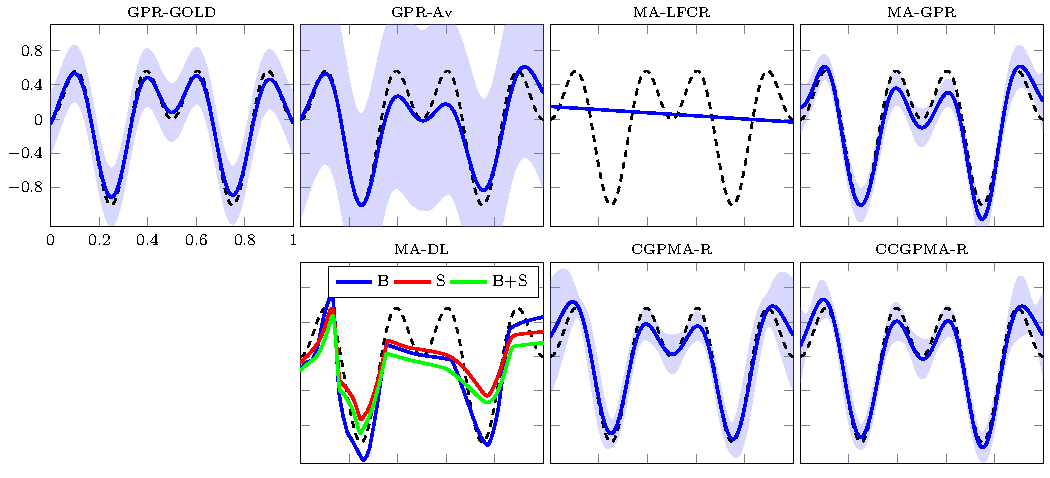
\includegraphics[width = \textwidth]{Figures/SinReg.pdf}
	\caption{Fully synthetic dataset results. We compare the prediction of our CCGPMA-R($R^2=0.9438$), and CGPMA-R($R^2=0.9280$) with the theoretical upper bound GPR-GOLD($R^2=0.9843$) and lower bound GPR-Av($R^2=0.8718$), and state-of-the-art approaches, MA-LFCR($R^2=-0.0245$), MA-GPR($R^2=0.9208$),  MA-DL-B($R^2=0.7020$), MA-DL-S($R^2=0.6559$), MA-DL-B+S($R^2=0.5997$). Note that we provided the Gold Standard in dashed lines. The shaded region in GPR-Av, MA-GPR, CGPMA-R, and CCGPMA-R indicates the area enclosed by the mean plus or minus two standard deviations. We remark that there is no shaded region for MA-LFCR, and DLMA since these approaches do not provide information about the prediction uncertainty.}
	\label{fig:FSReg}
\end{figure*}
\cref{fig:FSReg} shows the predictive performance of all methods in this first experiment. The results show two clear groups: those based on GPs (GPR-Av, MA-GPR, CGPMA-R, and CCGPMA-R), which expose the best performance in terms of the $R^2$ score, and those based on other types of approaches (MA-LFCR, and MA-DL), whose performance is not satisfactory. The behavior of MA-LFCR is poor, since it only can deal with linear problems. Besides, concerning MA-DL and its three variations (S, B, and S+B), we note that this approach, in general terms, has the capability of modeling the non-linearities present in the regression problem; however, MA-DL reaches a significantly low performance (even lower than the most naive approach, GPR-Av). To explain such an outcome, we remark that MA-DL comprises the introduction of an additional layer, the ``CrowdLayer'', which allows the training of neural networks, directly from the noisy labels of multiple annotators \cite{rodrigues2018deep}. However, such CrowdLayer provide a very simple codification of the annotators' performance to guarantee a low computational cost \cite{morales2019scalable1}; therefore, MA-DL does not provide a proper codification of the annotators' behavior. Among the GP-based methods, the proposed CCGPMA-R achieves the best performance in terms of $R^2$, followed closely by  CGPMA-R and MA-GPR. 

On the other hand, concerning the high performance of our CCGPMA-R (the best in terms of $R^2$ score), we hypothesize that such an outcome is a consequence that our approach offers a better representation of the labelers' behavior when compared with its competitors. To empirically support the above hypothesis, \cref{fig:ExpReg} shows the estimated error-variances for this first experiment; here, we only take into account the models that include these parameters in their formulations. From \cref{fig:ExpReg}, we note from the $R^2$ score and making a visual inspection that the approaches MA-LFCR and MA-GPR offer the worst representation for the annotator's performance, which is expected due to such models do not take into account the relationship between the annotators' performance and the input space. Conversely, CGPMA-R and CCGPMA-R clearly outperforms the models named previously. This outcome is a consequence that such two approaches compute such error-variances as functions of the input features, allowing for a better codification of the labelers' behavior. Besides, by making a visual inspection and analyzing the $R^2$ scores, CCGPMA-R performs better that CGPMA-R. The above is a consequence of that contrary to CGPMA-R, the CCGPMA-R codes the annotators' interdependencies, which improves the modeling of such performances as was empirically demonstrated in \cite{zhu2019unsupervised}. Finally, we remark that although our CCGPMA-R achieves the best representation of the annotators' performance, the result for Annotator 4 exhibit a lower performance in terms of $R^2$ score compared with the other labelers. Such an outcome is caused by the quasi-periodic behavior in the error-variances for those labelers, which cannot be captured by our approach because we are using a kernel RBF.

\begin{figure*}[!tb]
	\centering
	%\input{Figures/VarEXp.tex}
	\includegraphics[width = \textwidth]{Figures/VarEXp.pdf}
	\caption{Estimated values of error-variance for the five annotators in the \textit{fully synthetic} experiment. In the first column, from top to bottom, we expose the error-variances used to simulate the labels from each annotator. Furthermore, the subsequent columns from top to bottom present the estimation of such error-variances performed by state-of-the-art models that include these kinds of parameters in their formulation; moreover, the true error-variances are provided in dashed lines. The shaded region in CGPMA-R and CCGPMA-R indicates the area enclosed by the mean plus or minus two standard deviations. We remark that there is no shaded region for MA-LFCR, and MA-GPR since these approaches perform a fixed-point estimation for the annotators' parameters. Finally, we remark that the $R^2$ score between the true and estimated error variances are provided.}
	\label{fig:ExpReg}
\end{figure*}

\subsubsection{Results over semi-synthetic data}

\begin{table*}[!b]
	\centering
	%\tiny
	\scriptsize 
	\caption{Regression results in terms of $R^2$ score over \textit{semi synthetic datasets}. Bold: the highest $R^2$ excluding the upper bound GPR-GOLD.}
	\resizebox{.98\linewidth}{!}{
	\begin{tabular}{cccccccc}\toprule
		{Method} & {Auto} & {Bike} & {Concrete} & {Housing} & {Yacht} & {CT} & {Average}\\\midrule
		GPR-GOLD($M=40$)&$0.8604\pm0.0271$ & $0.5529\pm0.0065$ & $0.8037\pm0.0254$ & $0.8235\pm0.0419$ & $0.8354\pm0.0412$ & $0.8569\pm0.0055$ & $0.7888$\\ 
        GPR-GOLD($M=80$)&$0.8612\pm0.0279$ & $0.5603\pm0.0063$ & $0.8271\pm0.0230$ & $0.8275\pm0.0399$ & $0.8087\pm0.0423$ & $0.8648\pm0.0047$ & $0.7916$\\ 
        GPR-Av($M=40$)  &$0.8425\pm0.0286$ & $0.5280\pm0.0100$ & $0.7589\pm0.0279$ & $0.7834\pm0.0463$ & $0.7588\pm0.0498$ & $0.8070\pm0.0130$ & $0.7464$\\ 
        GPR-Av($M=80$)  &$0.8406\pm0.0304$ & $0.5397\pm0.0085$ & $0.7765\pm0.0274$ & $0.7903\pm0.0451$ & $0.7676\pm0.0535$ & $0.8167\pm0.0089$ & $0.7552$\\ 
        MA-LFCR         &$0.7973\pm0.0218$ & $0.3385\pm0.0051$ & $0.6064\pm0.0384$ & $0.7122\pm0.0509$ & $0.6403\pm0.0186$ & $\mathbf{0.8400\pm0.0014}$ & $0.6558$\\ 
        MA-GPR          &$0.8456\pm0.0281$ & $0.4448\pm0.0187$ & $0.7769\pm0.0367$ & $0.7685\pm0.0632$ & $0.7842\pm0.1027$ & $0.0105\pm0.0045$ & $0.6051$\\
        MA-DL-B         &$0.7766\pm0.0253$ & $0.5854\pm0.0107$ & $0.2319\pm0.0328$ & $0.5317\pm0.1005$ & $0.2089\pm0.0783$ & $0.6903\pm0.2689$ & $0.5041$\\ 
        MA-DL-S         &$0.7761\pm0.0279$ & $\mathbf{0.5828\pm0.0149}$ & $0.2363\pm0.0252$ & $0.5352\pm0.0948$ & $0.1822\pm0.0985$ & $0.9394\pm0.0257$ & $0.5420$\\ 
        MA-DL-B+S       &$0.7717\pm0.0239$ & $0.5816\pm0.0181$ & $0.2369\pm0.0322$ & $0.5330\pm0.0850$ & $0.1974\pm0.0895$ & $0.5517\pm0.2316$ & $0.4787$\\ 
        CGPMA-R($M=40$) &$0.8474\pm0.0221$ & $0.5464\pm0.0069$ & $0.8169\pm0.0231$ & $0.7946\pm0.0498$ & $0.7545\pm0.1029$ & $0.8236\pm0.0132$ & $0.7639$\\ 
        CGPMA-R($M=80$) &$0.7768\pm0.0708$ & $0.5560\pm0.0074$ & $0.8190\pm0.0254$ & $0.8058\pm0.0493$ & $0.8230\pm0.0760$ & $0.8371\pm0.0104$ & $0.7696$\\ 
        CCGPMA-R($M=40$)&$0.8563\pm0.0247$ & $0.5284\pm0.0117$ & $0.7976\pm0.0270$ & $0.7994\pm0.0462$ & $0.8436\pm0.0507$ & $0.8219\pm0.0062$ & $0.7745$\\ 
        CCGPMA-R($M=80$)&$\mathbf{0.8578\pm0.0244}$ & $0.5467\pm0.0069$ & $\mathbf{0.8220\pm0.0259}$ & $\mathbf{0.8110\pm0.0453}$ & $\mathbf{0.8476\pm0.0544}$ & $0.8252\pm0.0083$ & $\mathbf{0.7850}$\\\bottomrule
	\end{tabular}}
	\label{tab:SSRegResults}
\end{table*}
\cref{tab:SSRegResults} shows the results the experiment with \textit{semi synthetic dataset}. On average, our CCGPMA-R  exhibits the best generalization performance in terms of the $R^2$ score. On the other hand, regarding its GPs-based competitors (GPR-Av, MA-GPR, and CGPMA-R), we first note that the performance of CGPMA-R exhibit a similar (but lower) performance than CCGPMA-R. The above is a consequence of that conversely to CGPMA-R our CCGPMA-R model the annotators' interdependencies. Secondly, the intuitive lower bound GPR-Av exhibits a significantly worse prediction than our approaches. On the other hand, we remark the behavior of MA-GPR, which is lowest compared with its GPs-based competitors, even far worse than the supposed lower bound GPR-Av. The key to this abnormal outcome lies in the formulation of this approach; MA-GPR models the annotators' behavior by assuming that their performance does not depend on the input features and considering that the labelers make their decisions independently, which does fit the process that we use to simulate the labels for this experiment.
Next, we analyze the results concerning the linear model MA-LFR; attained to the results, we note that this approach's prediction capacity is far lower than our approaches; the above outcome suggests that there may exist a non-linear structure in most databases. However, we highlight a particular result for the dataset CT, where MA-LFCR exhibits the best performance defeating all its competitors based on non-linear models. From the above, we intuit that the CT dataset may have a linear structure. To confirm this supposition, we perform an additional experiment over CT by training a regression scheme based on LR with the actual labels (we follow the same scheme as for GPR-GOLD). We obtain an $R^2$ score equal to $0.8541$ (on average), which is close to the results obtained by GPR-GOLD. Thus, we can elucidate that there exists a linear structure in the dataset CT. Finally, we analyze the results for the DL-based models. Similar to the experiments over \textit{fully synthetic datasets}, we note a considerable low prediction capacity; in fact, they are even defeated by the linear model MA-LFR. Again, we attribute this behavior to the fact that the CrowdLayer (used to manage the data from multiple annotators) does not offer a suitable codification of the labelers' behavior. Nevertheless, taking the above into account, we observe an unusual result in the dataset Bike, where the DL-based approaches offer the best performance, even defeating the supposed upper-bound GPR-GOLD. To explain that, it is necessary to analyze the meaning of the target variable in such a dataset. Regarding to the description of this dataset,\footnote{Such description can be found in https://archive.ics.uci.edu/ml/datasets/bike+sharing+dataset} the target variables indicate the count of total rental bikes, including both casual and registered in a day. The above suggests that there may exist a quasi-periodic structure in the dataset, which cannot be captured by the GPR-GOLD since it uses a non-periodic kernel (it uses the RBF kernel). To support our suppositions, an additional experiment was performed over this dataset by training the model GPR-GOLD with the kernel defined as follows. 
\begin{align}\label{eq:Pkernel}
\kappa(\ve{x}_n, \ve{x}_{n^{\prime}}) = \varphi \exp \left[  - \frac{1}{2}\sum_{p=1}^{P}\left( \frac{\sin(\frac{\pi}{T_p} (x_{p,n}- x_{p,n^{\prime}}) )}{l_p}\right)^2 \right],
\end{align}
where $\varphi\in \Real$ is the variance parameter, $l_p\in (\Real^{+})$ is the length-scale parameter for the $p$-th dimension, and $T_p\in (\Real^{+})$ is the period for the $p$-th dimension. Therefore, we obtain an $R^2$ score equal to $0.5952$ (on average), which is greater than the obtained by the DL-based approaches, indicating a quasi-periodic structure in the Bike dataset as we had supposed.

\subsubsection{fully real data}
Finally, we use the \textit{fully real datasets}, which present the most challenging scenario, where both the input samples and the labels come from real-world applications. 
\begin{table}[!htb]
	\centering
	%\tiny
	\scriptsize 
	\caption{Regression results in terms of $R^2$ score over \textit{fully real dataset}. Bold: the highest $R^2$ excluding the upper bound GPR-GOLD.}
	\resizebox{.3\linewidth}{!}{
	\begin{tabular}{cc}\toprule
		{Method} & {Music}\\\midrule
		GPR-GOLD($M=40$)&$0.4704$\\
        GPR-GOLD($M=80$)&$0.4889$\\
        GPR-Av($M=40$)  &$0.2572$\\
        GPR-Av($M=80$)  &$0.2744$\\
        MA-LFCR         &$0.1404$\\
        MA-GPR          &$0.0090$\\
        MA-DL-B         &$0.2339$\\
        MA-DL-S         &$0.2934$\\
        MA-DL-B+S       &$0.3519$\\
        CGPMA-R($M=40$) &$0.3345$\\
        CGPMA-R($M=80$) &$0.3531$\\
        CCGPMA-R($M=40$)&$0.3337$\\
        CCGPMA-R($M=80$)&$\mathbf{0.3872}$\\\bottomrule
	\end{tabular}}
	\label{tab:FSRegResults}
\end{table}
\cref{tab:FSRegResults} outlines the achieved performances. We remark that our CCGPMA-R with $M=80$ obtains the best generalization performance in terms of $R^2$ score. Further, as theoretically expected, its performance lies between that of GPR-GOLD and GP-Av. 
Moreover, regarding the GPs-based competitors (MA-GPR and CGPMA-R), we note that similarly to previous experiments, our CGPMA-R is just a bit lower than CCGPMA-R, which is due to both frameworks estimate the annotators' performances as functions of the input features. On the other hand, MA-GPR exhibits the worst prediction capability with a $R^2$ close to zero. We suppose the above is a symptom of overfitting, which can be confirmed due to the training $R^2$ score for MA-GPR is $0.4731$, which is comparable with GPR-GOLD. Conversely, the linear approach MA-LFCR exhibits the second-lowest performance and performs worse than the theoretical lower bound GP-Av, which indicates a non-linear structure in the Music dataset. Finally, analyzing the results from the deep learning approaches, we note that the variation MA-DL-B+S exhibit a similar performance compared with our CGPMA-R; however, it is slightly lower than than our CCGPMA-R. We highlight that despite the capacities of deep learning, our approach CCGPMA-R offers a better representation of annotators' behavior, unlike the deep learning approaches, which measure such performance using a single parameter.\\
On the other hand, we observe that all regression models presented a lower generalization performance than previous results (see Table V in the paper) over the same dataset. The above is a repercussion of solving a multi-class classification problem with regression models.

\bibliographystyle{IEEEtran}
\footnotesize
\bibliography{refs}
\end{document}